\documentclass[10pt]{report} 
\usepackage[utf8]{inputenc}
\usepackage[T1]{fontenc}
\usepackage[ngerman]{babel}
\usepackage{hyperref}
\usepackage[dvipsnames]{xcolor}
% ----------------------------

% ----------------------------
% Pakete - Bilder und Symbole 
% ----------------------------

\usepackage{graphicx}          % \includegraphics (pdf-Version)
\usepackage{amssymb}           % AMS - Symbole
%\usepackage{amsmath}          % AMS - Umgebungen + Befehle (\begin{cases}...\end{cases},\pmatrix)

% ----------------------------
% Pakete - Format und Sprache
% ----------------------------

\usepackage[paper=a4paper,left=2.5cm,right=2.5cm,top=2cm,bottom=2.5cm]{geometry} % Formatierung
\usepackage[ngerman]{babel}    % Deutsche Bezeichnungen und Trennung nach neuer Rechtschreibung
\usepackage[T1]{fontenc}       % Trennen mit Umlauten
%\usepackage[latin1]{inputenc} % Umlaute direkt im Text (ISO 8859-1 UNIX-Systeme)
%\usepackage[utf8]{inputenc}   % Umlaute direkt im Text (MS-Windows)

% ----------------------------
% Pakete - Feineinstellungen
% ----------------------------

\usepackage{courier}           % Courier Schrift in verb-, verbatim- und listing-Umgebungen
%\usepackage{cmbright}         % Schriften-Gruppe im Text [cmbright, mathpazo (Palatino), times]
%\usepackage{hyperref}         % Links im Inhaltsverzeichnis und \url
%\usepackage{microtype}        % Bessere Darstellung: margin + extra kerning, expansion, tracking, and spacing
\usepackage{titlesec}          % Packet zur Anpassung der Titel der Kapitel
\titleformat{\chapter}[block]{\bfseries\LARGE}{\thechapter}{2.75ex}{}[\vspace{1ex}\titlerule]

% ----------------------------
% Sonstiges
% ----------------------------

\usepackage{nicefrac}
\usepackage{mathtools}


% ----------------------------
% Parameter
% ----------------------------

\linespread{1.05}              % Zeilenabstand einstellen
\setlength{\parindent}{0pt}    % Global \noindent
\setlength{\parskip}{5pt}      % Inhaltsverzeichnis + Platz zwischen Titel und Text

% ----------------------------
% Eigene Definitionen
% ----------------------------

\newcommand{\qed}{\ensuremath{\square} } % Statt q.e.d. ein kleines Quadrat
\newtheorem{Definition}{Definition}[section]
\newtheorem{Theorem}{Theorem}[section]
\newtheorem{Beispiel}{Beispiel}[section]
\newtheorem{Algorithmus}{Algorithmus}[section]
\newtheorem{Bemerkung}{Bemerkung}[section]
\newenvironment{Beweis}[1][Beweis]{\begin{trivlist}\item[\hskip \labelsep {\textit{#1 }}]}{\end{trivlist}
\hfill\qed}

% ----------------------------
% Quellcode-Listings
% ----------------------------

\usepackage{listings}
\lstset{
language    = python,
basicstyle  = \ttfamily, 
frame       = single,
numbers     = left, 
numberstyle = \scriptsize
}
\usepackage{float}
\newfloat{listing}{htbp}{scl}[chapter]
\floatname{listing}{Listing}

% ----------------------------

% ----------------------------

% ----------------------------
\begin{document}
% ----------------------------

% ----------------------------
\begin{titlepage}
% ----------------------------
\begin{center}\  

\vfill

\includegraphics[width=0.6\textwidth]{./pic/Logo_h_da}
\vfill
Fachbereich Mathematik und Naturwissenschaften\\
Fachbereich Informatik\\
Studiengang Data Science
\vfill
{\LARGE Data Science Projekt} \\[0.5cm]
\vfill
{\Huge Erkennung von Makulaödemen \\
durch maschinelles Lernen}
\vfill

Vorgelegt von  

\begin{tabular}{ll}
Heiko\ Raible & Matrikelnummer : \ 769082 \\
Corinna Erika\ Rentschler  & Matrikelnummer : \ 769282 \\
Svenja Sophia\ Schuder & Matrikelnummer : \ 769277 \\
Thi Nhat Le\ Pham  & Matrikelnummer : \ 770407 \\
\end{tabular}

am  \today

\vfill
\begin{tabular}{ll}
Referent     & Prof.\ Dr. \ Arnim Malcherek \\
Referent   & Prof.\ Dr. \ Horst Zisgen
\end{tabular}
\vfill
\end{center}
% ----------------------------
\end{titlepage}
% ----------------------------

% ----------------------------
\begin{abstract} 
% ----------------------------

Ziel des Projektes war es, auf einem System der Uniklinik Münster über maschinelle Lernverfahren Makulaödeme auf dort durchgeführten OCT-Scans zu erkennen, die Größe dieser zu vermessen und diese Informationen in die in der Uniklinik verwendeten Software Fidus einzubinden.

Hierbei war die Grundidee zur Umsetzung der maschinellen Lernverfahren ein zweistufiges Verfahren: Ein Efficient-Net als Vorfilter sowie ein Mask-R-CNN als Segmentierungsmodell. Beide Modelle einzeln liefern zufriedenstellende Ergebnisse. Da das Segmentierungsmodell einzeln zu besseren Ergebnissen als die Kombination beider Modelle im Rahmen eines zweistufigen Verfahrens führt, ist im finalen Prototypen nur dieses Modell eingebunden.

Ein Qualitätsgewinn der Vorhersagen durch die Klassifikation als Vorfilter wurde in Frage gestellt, scheint jedoch vielversprechend und Bedarf weiterer Untersuchungen.

Mit dem Mask R-CNN Segmentierungsmodell sowie einem Skript, mithilfe dessen die Ergebnisse des Modells in die Fidus Software eingebunden wird, werden die gesetzten Ziele zufriedenstellend erreicht und beweisen somit eine technische Anwendbarkeit in der Praxis.

% ----------------------------
\end{abstract}
% ----------------------------

% ----------------------------
\tableofcontents
% ----------------------------



% ---------------------------------------------------------------------------------------------------------
\chapter{Einleitung}
% ----------------------------
Im Rahmen des Data Science Projektes an der Hochschule Darmstadt wird, in Kooperation mit der Klinik für Augenheilkunde an der Uniklinik Münster, an Methoden zur Diagnostik von Erkrankungen des Auges geforscht. 

In bereits mehreren Vorgängerprojekten wurden, mit Hilfe von Machine-Learning-Verfahren (ML-Verfahren), Methoden zur Diagnostik solcher Erkrankungen, wie der Glaukomerkennung, entwickelt.

Die Erkennung und Behandlung von Makuladegeneration ist eine der Diagnostiken, die die Augenärzte an der Uniklinik Münster durchführen. Im Praxisalltag werden für die Erkennung von Makulaödemen Aufnahmen des Auges, sogenannte Optische Kohärenz-Tomographien (OCT), gemacht. Nach Sichtung der OCT-Scans durch den Arzt wird anschließend die entsprechende Therapie gewählt. Im Rahmen dieses Projektes soll ein Verfahren zur Erkennung von Makulaödemen entwickelt werden, um diesen Vorgang zu unterstützen.

\section{Zielsetzung}

Ziel des Projektes ist es, Makulaödeme auf OCT-Scans zu erkennen.
Durch maschinelles Lernen soll ein Verfahren entwickelt werden, das in der Lage ist, Ödeme zuverlässig auf OCT-Scans zu erkennen. 
Das Verfahren soll Ärzte bei der Diagnostik unterstützen, indem die Erkennung von Ödemen automatisiert nach der Untersuchung von Patienten durchgeführt wird.

Neben der Erkennung von Ödemen ist es im medizinischen Sinne bedeutend, inwiefern sich bei Patienten vorliegende Ödeme entwickeln. Zu diesem Zweck soll neben der Erkennung eine Verlaufskontrolle entwickelt werden, zu der die Größe der Ödeme ermittelt wird. Über die Größe erhalten Ärzte Aufschluss darüber, wie weit eine Erkrankung bereits fortgeschritten ist.

Um die praktische Anwendbarkeit bei der Diagnostik zu demonstrieren, soll das entwickelte Verfahren auf den Computersystemen des Uniklinikums installiert werden. 
Ziel ist es hier den Prototypen in das bestehende Softwaresystem zu integrieren, um einen ersten technischen Durchstich zu erlangen.

\newpage
\section{Vorgehen und gewählte Methoden}

Um die Ziele wie im vorherigen Abschnitt beschrieben zu erreichen, werden die Aufgaben in drei Schritte aufgeteilt. Als erstes die Vorverarbeitung der Daten, anschließend die Implementierung der ML-Verfahren und zuletzt das Vereinen dieser in einem Prototypen auf dem Zielsystem. Die einzelnen Schritte werden in folgenden Kapiteln genauer beschrieben. 

Als Testdaten hat das Uniklinikum 34.943 OCT-Bilder zur Verfügung gestellt, von denen einige ein Ödem aufweisen. 
Für das Trainieren des gewählten ML-Verfahrens ist es notwendig, neben den OCT-Bildern auch die Lage und Form der Ödeme als Information mit einzugeben. 
Um das zu ermöglichen werden die Ödeme auf den vorhandenen OCT Bildern zunächst händisch segmentiert. 

Der nächste Schritt ist es, die OCT-Bilder nach Existenz von Ödemen zu klassifizieren. Hierzu dient ein Convolutional Neural Network (CNN) der EfficientNet Architektur. Neben der reinen Klassifizierung von Ödemen soll auch die Größe der Ödeme bestimmt werden. Dazu ist ein weiteres Modell nötig, das nicht nur das Vorhandensein von Ödemen bestimmt, sondern auch deren Lage auf den OCT-Bildern detektieren kann. Hierfür wird auf Basis eines vortrainierten Mask R-CNN ein Modell zur Instance Segmentation von Ödemen erstellt.

Schließlich werden die beiden Modelle in einem Prototypen vereint, der in die Systeme des Uniklinikums eingebettet wurde. Der somit erreichte Durchstich zeigt die technische Machbarkeit der Integration von ML-Verfahren für diese Problemstellung auf und vermittelt den Ärzten einen ersten Eindruck, wie die Anwendung in der Praxis aussehen könnte. 
% ----------------------------


% ---------------------------------------------------------------------------------------------------------
\chapter{Datenvorverarbeitung}
% ----------------------------
\section{Die Daten}

Die zur Verfügung gestellten Daten bestehen aus 34.943 Bildern, wobei jeweils 25 Bilder einem Auge zugehörig sind. Auf einem Bild ist sowohl die Draufsicht des ganzen Auges, als auch jeweils einer der 25 Querschnitte zu sehen.

\begin{figure}[H]
\centering
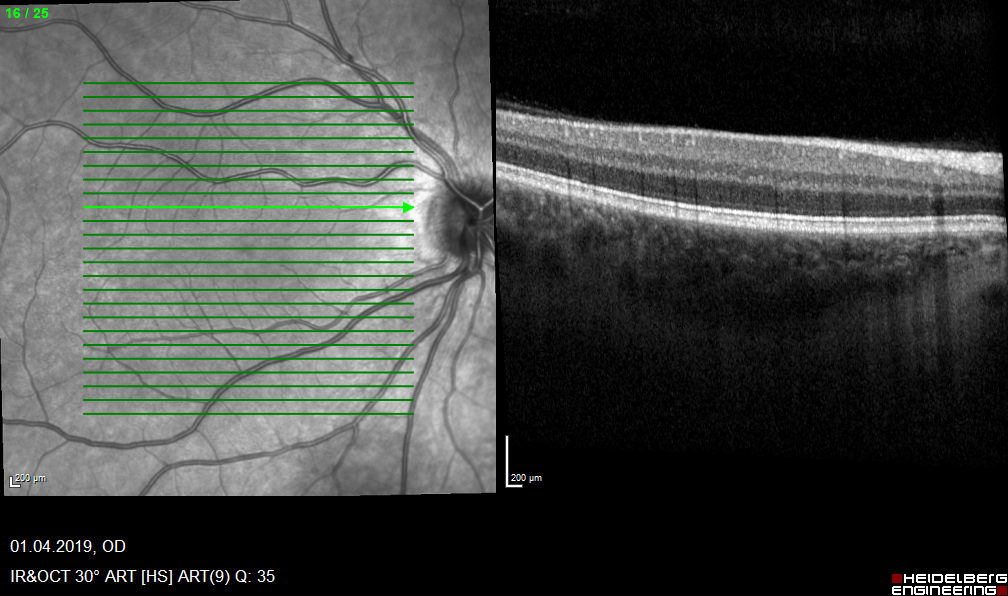
\includegraphics[width=0.7\textwidth]{./pic/Datenvorverarbeitung/OCT-Scan.png}
\caption{\label{fig:octscan}OCT Scan einer Schicht.}
\end{figure}

Die Draufsicht (Abb. \ref{fig:octscan} links) kann bei der Interpretation der Querschnitte hilfreich sein - der Großteil der relevanten Informationen für eine Ödemerkennung befindet sich jedoch auf den Querschnitten (Abb. \ref{fig:octscan} rechts).

In diesem Projekt werden die Querschnitte dennoch aus den Bildern extrahiert und die Draufsicht verworfen, um die Informationsdichte für das maschinelle Lernverfahren zu erhöhen. Dies wird automatisiert über die PIL Python library realisiert.

\section{Labeling}

Um den gewählten Supervised Learning Verfahren das Lernen aus den Daten zu ermöglichen, ist es notwendig, dass zuvor jedes Bild händisch klassifiziert und segmentiert wird. Für die Segmentierung dient das Tool VGG Image Annotator \cite{24}. Das Tool besteht aus einer browserbasierten Anwendung, mit der man die Bilder laden und Bereiche per Maus markieren kann (vgl. Abb. \ref{fig:vgg}) .

\begin{figure}[H]
\centering
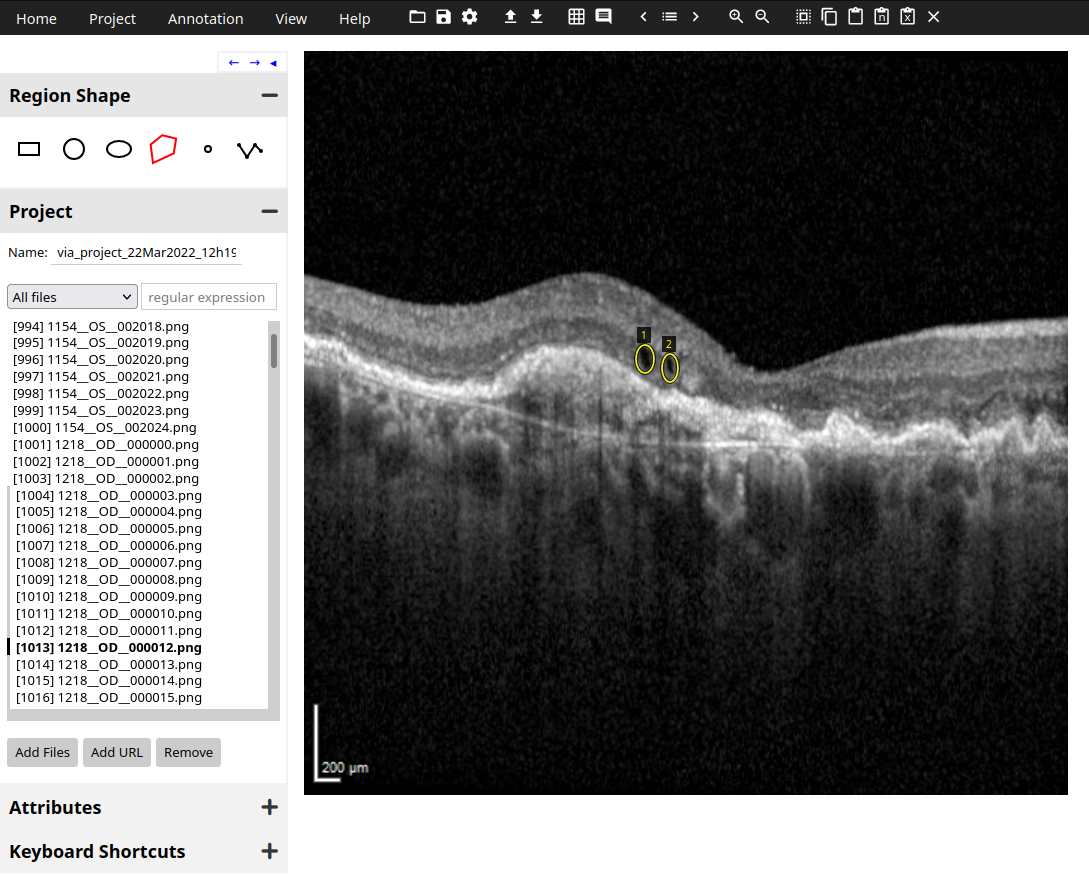
\includegraphics[width=0.7\textwidth]{./pic/Datenvorverarbeitung/VGG.png}
\caption{\label{fig:vgg}Labeln und Segmentieren eines Bildes im VGG Image Annotator}
\end{figure}

Um die Klassifizierung aus der Segmentierung zu gewinnen werden Klassenlabel für alle Bilder mit segmentierten Bereichen auf True und alle Bilder ohne segmentierte Bereiche auf False gesetzt. Dies ergibt 2.624 Bilder mit Ödem und 32.319 Bilder ohne Ödem. Dieses unausgewogene Verhältnis der Klassen und die geringe Menge an positiven Bildern bringt einige Probleme mit sich, wie einen Mangel an Trainingsdaten für die Segmentierung, welche nur auf positiven Bildern arbeitet, oder eine erschwerte Evaluierung.

Weitere Gegebenheiten die beim Labeling Verfahren die Qualität verringern sind ein Labeling basierend auf Laienwissen, unterschiedliche Labeler ohne stringende Labeling Richtlinien und ein Zeitmangel für die große Anzahl an Bildern.

\section{Datensätze}

\subsection{Datensätze für die Klassifikation}
Die gelabelten Bilder müssen nun noch in zwei getrennte Datensätze eingeteilt werden: Jene Daten die für das Training verwendet werden sowie Daten, welche für die anschließende Evaluierung der Performance auf ungesehenen Daten zurückgehalten werden. Aufgrund des unausgewogenen Verhältnisses der Bilder mit und ohne Ödem wird ebenfalls darauf geachtet, dass die Bilder stratifiziert auf die Datensätze aufgeteilt werden, also das Verhältnis an positiven und negativen Bildern auf beiden Datensätzen gleich gehalten wird. In Abb. \ref{fig:dataset_distribution} wird die Aufteilung der Trainings- und Testdaten für das Training und Testen des Klassifizierers vorgestellt.

\begin{figure}[H]
\centering
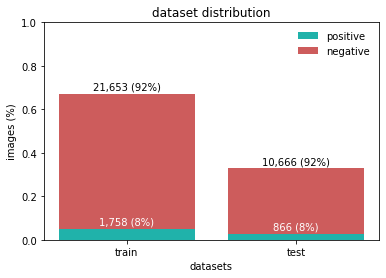
\includegraphics[width=0.6\textwidth]{./pic/Datenvorverarbeitung/classes.png}
\caption{\label{fig:dataset_distribution}Verteilung der Trainings- und Testdaten für die Klassifikation. Links ist der Trainingsdatensatz, rechts der Testdatensatz zu sehen. Die Anteile der Bilder mit Ödem (positiv) sind türkis dargestellt, die Anteile der Bilder ohne Ödem (negativ) sind rot eingefärbt.}
\end{figure}

\subsection{Datensätze für die Segmentierung}
Das Training der Segmentierung wird ausschließlich auf Bildern mit Makulaödemen (positiv) vorgenommen. Daher wurden separate Trainings-und Testdatensätze für die Segmentierung erstellt.\newline
Da im Training ausschließlich positive Bilder verwendet werden können und der Datenumfang entscheidend für den Trainingserfolg sein kann, wurde ein Trainings-/Testsplit gewählt, bei dem ein Großteil der Bilder im Trainingsdatensatz verwendet werden.
% Test: insg. 50 pos, alle negative
% Trainig: alle positiven Bilder minus 50


Um das Mask R-CNN trainieren zu können, werden als Input-Daten neben den Bildern auch die Masken der Ödeme im Bild benötigt. Dafür wird für alle mit dem VGG Image Annotator von Hand segmentierten OCT-Bilder, die Fläche der Ödeme berechnet und anschließend über die Pixelmenge innerhalb der Fläche die Maske erstellt. 
Die Masken, die im Training übergeben werden, enthalten nun nur noch die Pixelfläche der segmentierten Ödeme eines OCT-Scans. Je nachdem wie viele Flüssigkeitsansammlungen auf einem OCT-Scan von Hand segmentiert wurden, kann eine Maske ein oder mehrere Flächen enthalten. 
In Abbildung \ref{input_mrcnn} sind beispielhafte Input-Daten abgebildet. 

\begin{figure}[H]
\centering
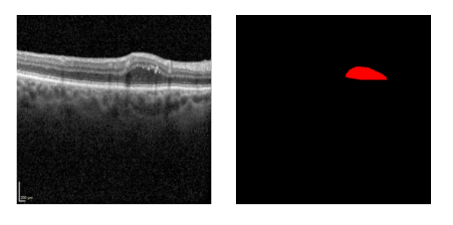
\includegraphics[width=100mm,scale=1.5]{pic/Segmentierung/input_mrcnn.png}
\caption{\label{input_mrcnn}Input-Daten des Mask R-CNN (Links: OCT-Bild, Rechts: Maske des Ödems)}
\end{figure}

Für das Training wurden die Daten in Trainings- und Validierungsdatensatz in einem Verhältnis von 80:20 aufgeteilt. Die beiden Input-Datensätze bestehen wiederum aus den OCT-Bildern sowie deren Masken (vgl. Abb.\ref{aufteilung_data}). 

Da für das Trainieren nur die OCT-Bilder auf denen sich ein Ödem befindet verwendet werden können, werden insgesamt 5598 Bilder aus dem gesamten Datensatz von 34.948 OCT-Bildern berücksichtigt. 
Von dem Trainingsdatensatz werden 50 Bilder entnommen, die später für das Testen des Modells verwendet werden. 
Somit befinden sich 4439 Bilder im Trainingsdatensatz und 1109 im Validierungsdatensatz. 

Das Mask R-CNN wurde mit den beschriebenen Datensätzen für 10 Epochen auf Cloud-Ressourcen von Amazon-Web-Services trainiert. Im folgenden Abschnitt wird die Verwendung von AWS näher beschrieben. 


\begin{figure}[H]
\centering
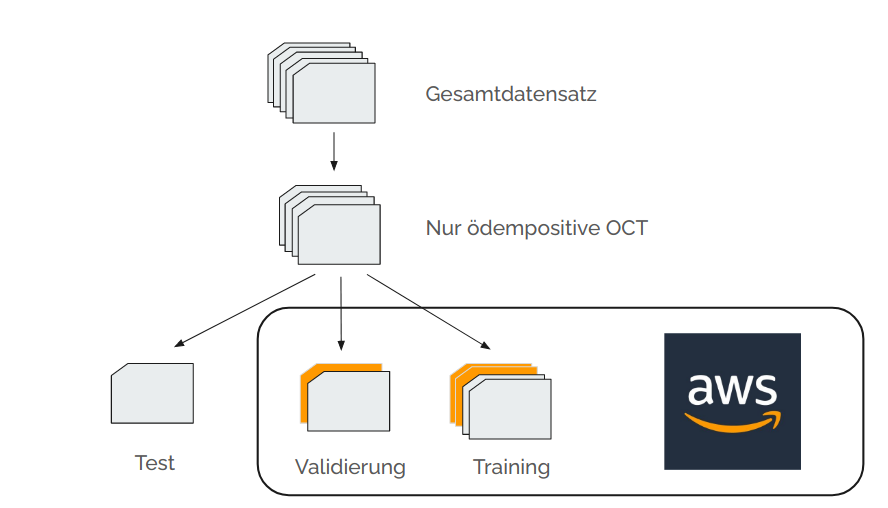
\includegraphics[width=0.7\textwidth]{pic/Segmentierung/training_segmentation.png}
\caption{\label{aufteilung_data}Aufteilung der OCT-Bilder für das Training des Mask R-CNN}
\end{figure}

\section{Training auf AWS}

Da aufgrund der hohen Datenmenge eine hohe Rechenkapazität notwendig ist, wird das Training der CNN jeweils für die Klassifikation und die Segmentierung auf Cloud-Ressourcen von Amazon Web Services durchgeführt. 
Das Training würde auf privaten Rechnern aufgrund der zu geringen Rechenkapazität schlicht von zu langer Dauer sein.
Die genutzte p2.xlarge Instanz von AWS verfügt über eine K80-GPUs von NVIDIA, 4 CPUs und 61 GB RAM, und ist somit speziell für die Berechnung von Deep Learning Verfahren ausgelegt.  (vgl. \cite{15}) 
Als persistentes Speichermedium, auf dem die Daten für das Training sowie dessen Ergebnisse abgelegt werden, wird ein S3 Bucket von AWS verwendet.






% ---------------------------------------------------------------------------------------------------------
\chapter{Klassifikation}
% ----------------------------
\section{Architektur}

Convolutional Neural Network, kurz CNN bzw. ConvNet ist eine Untergruppe von Artificial Neural Network (ANN),  die sich auf die Klassifizierung von Daten gitterartiger Topologie wie Bilder spezialisiert. Wie das menschliche Gehirn kann CNN eine riesige Menge an Daten aus einem Bild extrahieren und verarbeiten, weshalb es zur Modellierung des menschlichen Sehens von Bedeutung ist. 

In den folgenden Unterabschnitten wird die allgemeine Architektur eines CNNs (\ref{CNN}), die logistische Regression zur Klassifikation binärer Zielvariablen im CNN (\ref{subsec:logReg}) und das EfficientNet als final gewählte Architektur (\ref{EfficientNet}) erklärt; englische Fachbegriffe werden im Verlauf bewusst beibehalten und nicht ins Deutsche übersetzt, um Präzision zu verleihen.

% ----------------------------
\subsection{CNN} \label{CNN}
% ----------------------------
CNN umfasst eine Klasse von Architekturen, die sich in der Anzahl der Layers, Anzahl der Filter, Filtergröße usw. unterscheiden. Dennoch ist jedes CNN hauptsächlich gekennzeichnet durch drei Layer: Convolutional Layer, Pooling Layer und Fully Connected Layer. Die ersten beiden Layer dienen zur Feature Extraction und Feature Learning und die letzte Layer ist verantwortlich für die eigentliche Klassifizierung. Eine Layer besteht dabei aus einer Sammlung von Neuronen und besitzt ihre eigenen Gewichten und Biases.


\begin{figure}[H]
\centering
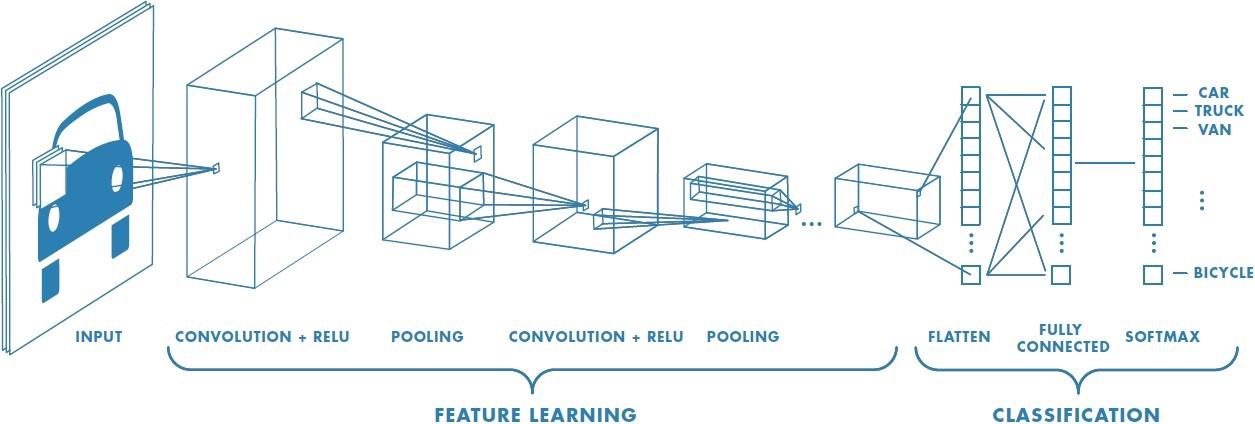
\includegraphics[width=0.8\linewidth]{pic/Klassifikation/CNN-Architektur.jpeg}
\caption{\label{pic:cnn} CNN Architektur}
\end{figure}



Nachfolgend werden die verschiedenen Layers eines allgemeinen CNNs, wie in der obigen Abbildung gezeigt, erläutert und anschließend der Trainingsalgorithmus eines CNNs präsentiert.
Die Arbeiten in \cite{1}, \cite{2}, \cite{3}, \cite{4} und \cite{5} dienen dabei als Grundlage für die nachstehende Darlegungen.

\subsubsection{Input}
Jedes Eingabebild wird durch eine Matrix bzw. Matrizen von Pixelwerten, auch als Tensor bezeichnet, repräsentiert. Es wird dabei zwischen einem farbigen, einem Graustufen bzw. einem Schwarz-Weiß-Bild unterschieden. Ein farbiges Bild wird durch drei Farbkanäle: rot, grün und blau, gekennzeichnet, wobei die Kanäle als 2D-Matrizen mit Pixelwerten zwischen 0 und 255 dargestellt werden. Weniger Speicherbedarf hat ein Graustufen-Bild, da dieses durch eine einzige 2D-Matrix, ebenfalls mit Pixelwerte zwischen 0 und 255, beschrieben wird. Noch weniger Speicher benötigt ein Schwarz-Weiß-Bild, welches nur Pixelwerte von 0 und 1 enthält. 

\subsubsection{Convolutional Layer} 
Das Eingabebild wird nun in die Convolutional Layer weitergegeben, in der dessen wesentliche Informationen (Features) extrahiert werden; man spricht hierbei von Feature Extraction. 

Die Convolutional Layer ist Kernbestandteil des CNNs und trägt den Hauptteil der Rechenlast des Netzwerkes. Sie  besteht aus linearen (Convolution) und nichtlinearen (ReLU) Operationen. Lineare bzw. Convolution Operationen sind für das eigentliche Feature Extraction verantwortlich, während nichtlineare Operationen schließlich angewendet werden, um der Rechenaufwand, vor allem in der Backpropagation, zu verringern.

Das Feature Extraction in der Convolution erfolgt durch die Matrixmultiplikation von zwei Matrizen; die eine ist der sogenannte Kernel und die andere ist das rezeptive Feld des Tensors, welche sich durch das Schieben über die Höhe und Breite des Tensors ergibt. In der unteren Abbildung \ref{pic:convolution} entspricht das rezeptive Feld dem orange-markierten Bereich im Input Tensor.

\begin{figure}[H]
\makebox[\linewidth]{%
  \begin{tabular}{ccc}
    &  &  \\
    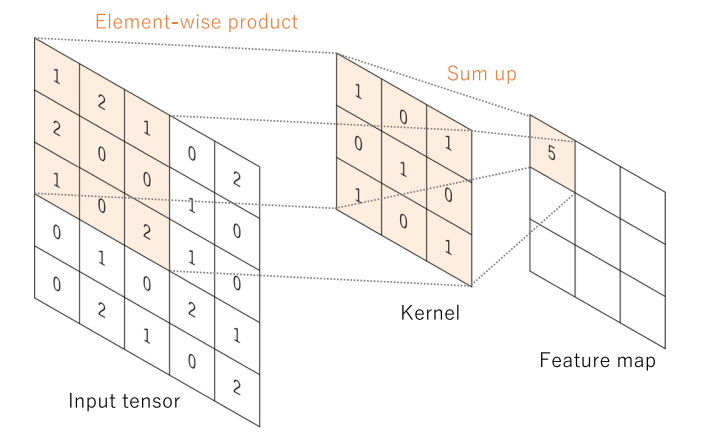
\includegraphics[width=0.28\linewidth]{pic/Klassifikation/convolution1.png}&
    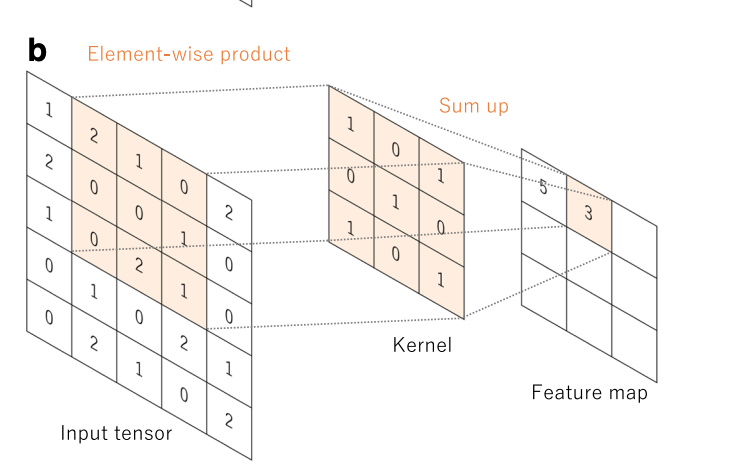
\includegraphics[width=0.28\linewidth]{pic/Klassifikation/convolution2.png}&
    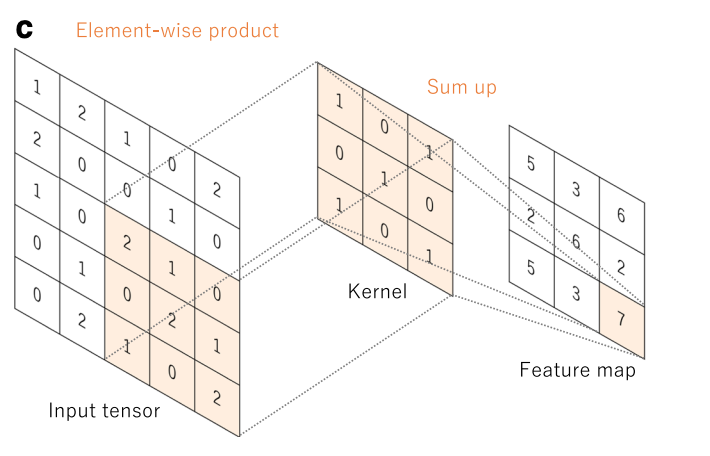
\includegraphics[width=0.28\linewidth]{pic/Klassifikation/convolution3.png}\\
  \end{tabular}%
}
 \caption{Convolution mit einem 3$\times$3-Kernel und Stride=1}
  \label{pic:convolution}
\end{figure}


Der Kernel ist in der Regel eine 3$\times$3, manchmal auch 5$\times$5 oder 7$\times$7 Matrix. Welche Features aus dem Tensor extrahiert werden, wird mit der Wahl der Kernels entschieden. Je mehr Kernels für die Convolution gewählt wird, desto mehr Informationen werden erfasst. Es ist jedoch anzumerken, dass mit der Genauigkeit auch die Rechenlast des Netzes ansteigt.


Die sich aus der Matrixmultiplikation ergebende Matrix heißt Feature Map. Ihre Größe wird durch drei Parameter bestimmt: Anzahl der Kernels, Stride und Padding (siehe \ref{def:FeatureMapDimCL}). Dabei gibt der Stride an, um wie viele Einheiten der Kernel über den Tensor vor jeder Matrixmultiplikation geschoben wird. Das Padding beschreibt das Auffüllen von Werte wie z.B Nullen (Zero-Padding) um den Tensor-Rand herum, um Informationsverlust zu vermeiden. Mit der Verwendung eines Zero-Paddings wird Convolution auch Wide Convolution genannt, während Narrow Convolution eine Convolution ohne Zero-Padding beschreibt.

\begin{Definition}[Dimension der Feature Map im Convolutional Layer] \label{def:FeatureMapDimCL}
Es seien ein Tensor der Dimension $n$$\times$$n$ und ein Kernel der Dimension $f$$\times$$f$ mit jeweils $p$ die Anzahl der Zerro-Padding Layers, $s$ die Größe des Strides und $z$ die Anzahl der Kernels gegeben, dann ist die Dimension der Feature Map im Convolutional Layer $m$$\times$$m$ gegeben durch: 
\begin{equation}
m \times m = (\frac{n+2p-f}{s} + 1) \times (\frac{n+2p-f}{s} + 1) \times z. \label{Dimension Feature Map im Convolutional Layer}
\end{equation}
\end{Definition}

Mit einer Aktivierungsfunktion werden die Werte der Feature Map nun auf einen bestimmten Bereich transformiert. ReLU ist aufgrund ihrer Performanz die meist verwendete Aktivierungsfunktion in der Hidden Layer von CNNs. Nach einer ReLU enthält die Feature Map nur positive Werte, da negative Werte jeweils durch eine Null ersetzt werden. Eine ReLU Aktivierungsfunktion sieht folgendermaßen aus.

\begin{figure}[H]
\centering
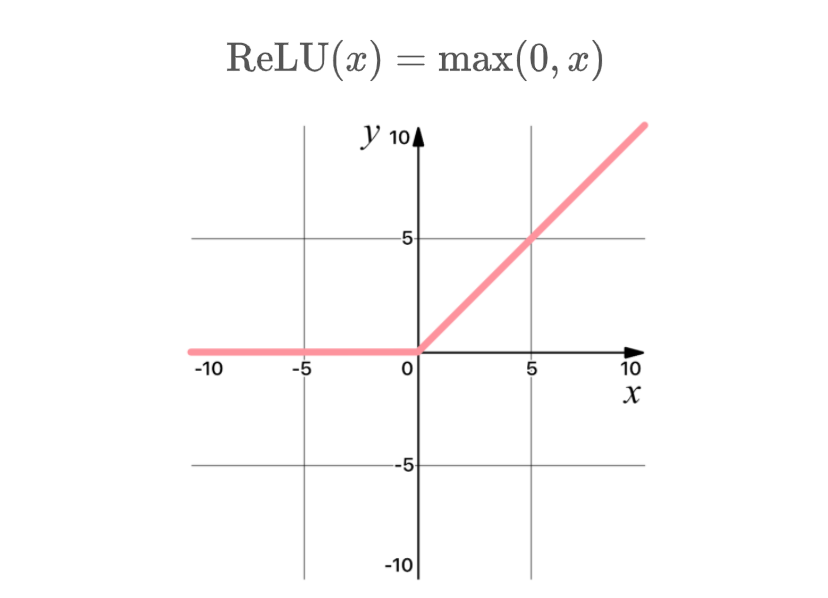
\includegraphics[width=0.5\linewidth]{pic/Klassifikation/ReLU.png}
\caption{\label{pic:ReLU} ReLU Aktivierungsfunktion}
\end{figure}

\subsubsection{Pooling Layer}
Die Feature Map aus der Convolutional Layer wird nun in die Pooling Layer zum weiteren Feature Extraction weitergeleitet. Mit dem Feature Extraction wird die Dimension der Feature Map reduziert und das Overfitting vermieden. Das Netz ist demnach invariant zu kleinen Transformationen,  Verzerrungen und Übersetzungen im Eingabebild. So können Objekte z.B. unabhängig von ihrer Lage im Bild richtig klassifiziert werden. Es gibt verschiedene Arten von Pooling, z.B. Max, Average oder Sum Pooling. In der Praxis zeigt sich das Max Pooling als performanter, weshalb es auch die meist verwendete Pooling Art ist.

Das Pooling funktioniert ähnlich wie die lineare Operation in der Convolutional Layer; auch hier wird ein Kernel über die Eingabematrix geschoben. Nur in der Berechnung der Ausgabewerte gibt es zur Convolutional Layer einen Unterschied. In jedem rezeptiven Feld der Eingabematrix entnimmt der Kernel, je nach Pooling Art, entweder das Maximum, das arithmetische Mittel oder die Summe der Werte des rezeptiven Feldes. Im Fall eines Max Poolings ergeben die Maxima der rezeptiven Felder die Ausgabematrix. Dies wird mit der unteren Abbildung \ref{pic:MaxPooling} veranschaulicht.

\begin{figure}[H]
\centering
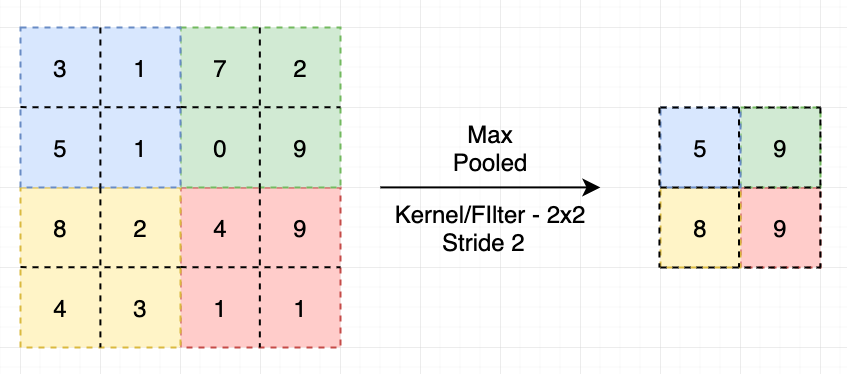
\includegraphics[width=0.5\linewidth]{pic/Klassifikation/MaxPooling.png}
\caption{\label{pic:MaxPooling} Max Pooling mit einem 2$\times$2-Kernel und Stride=2}
\end{figure}

Es gibt in der Regel kein Padding in der Pooling Layer. Die Ausgabematrix wird somit nur von der Dimension der Feature Map und der Größe des Strides beeinflusst. Die Dimension der Feature Map lässt sich, wie in \ref{def:DimFeatureMapPL} definiert, bestimmen.

\begin{Definition}[Dimension der Feature Map im Pooling Layer] \label{def:DimFeatureMapPL}
Es seien eine $n_{H}$$\times$$n_{W}$$\times$$n_{C}$ Eingabematrix (Feature Map nach Convolutional Layer) und ein $f$$\times$$f$ Kernel mit $s$ die Größe des Strides gegeben, dann ist die Dimension der Feature Map $m$$\times$$m$ im Pooling Layer  definiert mit: 
\begin{equation}
m_{H}\times m_{W}\times m_{C} =  (\frac{n_{H}-f}{s} + 1) \times (\frac{n_{W}-f}{s} + 1) \times n_{C}. \label{Dimension Feature Map im Pooling Layer}
\end{equation}
\end{Definition}

\subsubsection{Fully Connected Layer}
Die Feature Map aus der letzten Pooling Layer wird nun transformiert in einen eindimensionalen Vektor (man spricht hierbei auch von Flatten) und in die Fully Connected Layer übergeben. Die Fully Connected Layer ist selbst ein Neuronales Netz, dessen Architektur nach Fragestellung variiert.

Für eine Klassifikation mit binären Zielvariablen eignet sich die Logistische Regression, auf dessen Architektur im Abschnitt \ref{subsec:logReg} eingegangen wird. 

\subsubsection{Der CNN-Algorithmus}
Der Algorithmus des CNN lässt sich nach \cite{2} in fünf Schritten zusammenfassen:
\begin{enumerate}
\item Initialisiere Parameter, Gewichte und Kernels mit zufälligen Werten.
\item Folge der Forward Propagation durch alle Layers der Feature Extraction (Convolution + ReLU, Pooling Layer) in die Klassifikation (Fully Connected Layer) und berechne die ersten Klassenwahrscheinlichkeiten für jedes Objekt.
\item Berechne den Gesamtfehler der Wahrscheinlichkeiten mit:
\begin{equation}
Total Error = \sum \nicefrac{1}{2} (Target Probability - Output Probability) ^2. \label{Total Error}
\end{equation}
\item Folge der Back Propagation und berechne mit dem Gradientenverfahren die neuen, optimierten Parameter-, Gewichten- und Kernels-Werte.
\item Wiederhole die Schritte 2-4 für alle Bilder im Traning Set.
\end{enumerate}


% ----------------------------
\subsection{Logistische Regression} \label{subsec:logReg}
% ----------------------------
Das Konzept der Fully Connected Layer und der Optimierung der Parameter mittels Gradientenverfahren wird in diesem Unterabschnitt an der Logistischen Regression in Anlehnung an der Arbeit von Daniel Jurafsky und James H. Martin (s. \cite{6}) erklärt.



Im Wesentlichen kann die Architektur einer logistischen Funktion anhand von 4 Komponenten beschrieben werden: Feature Vektor, Aktivierungsfunktion (Sigmoid), Verlustfunktion (Cross-Entropy) und Optimierungsalgorithmus (Gradientenverfahren). Diese Komponenten werden im Folgenden genauer erläutert. 


\begin{figure}[H]
\centering
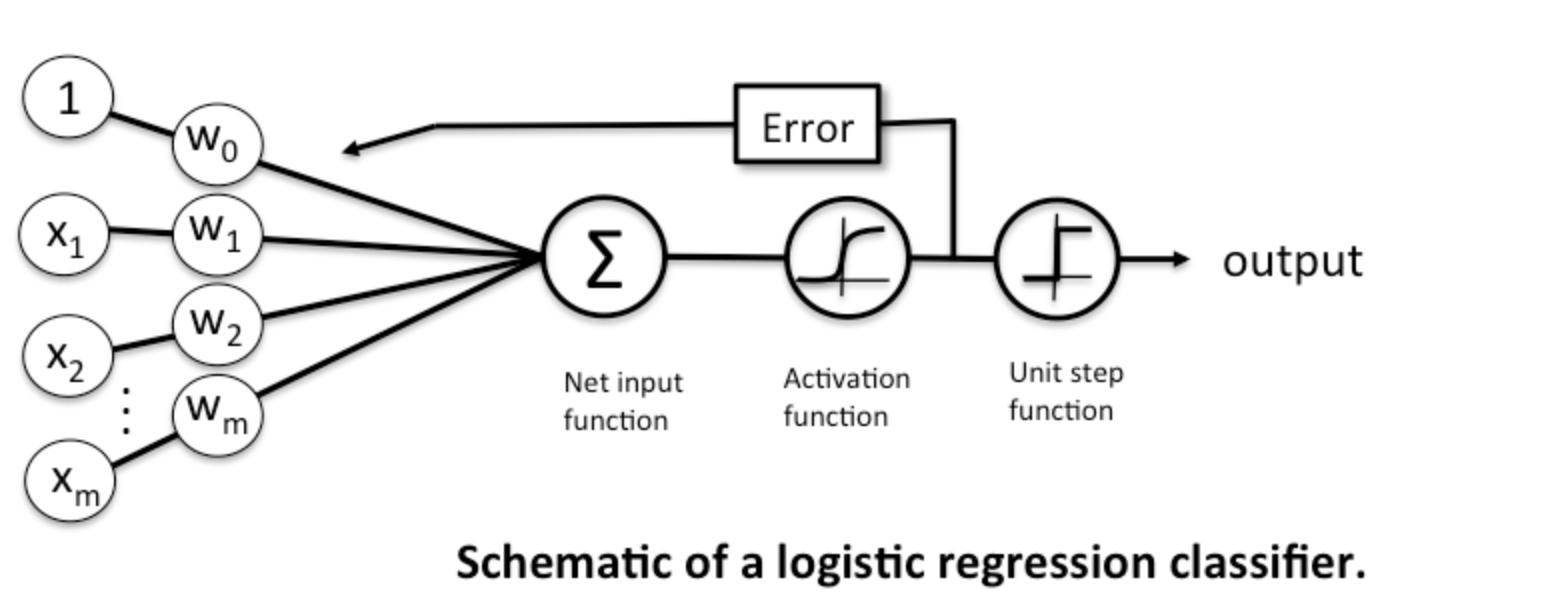
\includegraphics[width=0.5\linewidth]{pic/Klassifikation/LogRegSchema.png}
\caption{\label{pic:logreg} Logistische Regression}
\end{figure}



\subsubsection{Feature-Vektor}
Der eindimensionale Feature-Vektor [ $x_{1}$, $x_{2}$, ..., $x_{n}$ ], der durch das Flatten der Feature Map aus der letzten Pooling Layer entsteht, ist Input der Fully Connected Layer. 
Da jede Klasse von anderen Features charakterisiert wird, ist es von Bedeutung die Features entsprechend zu gewichten. Wir bezeichnen $z$ als die Multiplikation des Feature-Vektors mit dem Gewichten-Vektor [ $w_{1}$, $w_{2}$, ..., $w_{n}$ ] und anschließende Addition mit dem Bias $b$.
\begin{equation}
z = ( \sum\limits_{i=1}^{n} (w_i\cdot x_i)+b ). \label{z}
\end{equation}
Aufgrund ihres Intervalls ($-\infty$,$+\infty$) kann mit $z$ noch keine Entscheidung getroffen werden, ob das eingegebene Objekt zur Klasse 1 oder 0 gehört. Der Wertebereich von $z$ muss daher auf den Intervall [0,1] angepasst werden, womit der sich ergebende Wert als Wahrscheinlichkeit interpretiert werden kann. Die Entscheidungsfunktion anhand der Wahrscheinlichkeit sieht folgendermaßen aus:
\begin{equation}
decision(x) = \left\{
\begin{array}{ll}
1 & \textrm{if $P$($y=$1$|$$x$) $>$ 0.5 }  \\
0 & \, \textrm{otherwise}. \\
\end{array}
\right. 
 \label{decision function} 
\end{equation}


\subsubsection{Sigmoid Funktion}
Die Transformation von $z$ auf den Intervall  [0,1] erfolgt mit der Sigmoid-Funktion $\sigma(z)$. 
\begin{figure}[H]
\centering
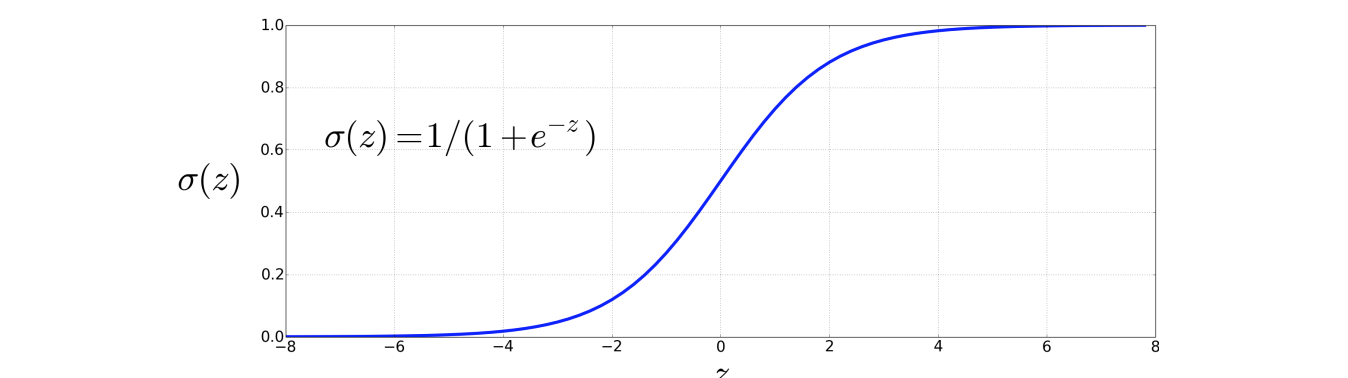
\includegraphics[width=0.7\linewidth]{pic/Klassifikation/sigmoid.png}
\caption{\label{pic:sigmoid} Sigmoid Aktivierungsfunktion}
\end{figure}

Damit der sich ergebende Wert aus $\sigma(z)$ als Wahrscheinlichkeit interpretiert werden kann, muss \begin{equation}
p(y=1) + p(y=0) = 1 \label{Wahrscheinlichkeit} 
\end{equation}
gelten. Dies ist dann der Fall, wenn:
\begin{equation}
p(y=1) =  \frac{1}{1+e^{-z} }  \label{p(y=1)}  
\end{equation}
und
\begin{equation}
p(y=0) =  1 - \frac{1}{1+e^{-z} }  \label{p(y=0)}  
\end{equation}
ist.


\subsubsection{Cross-Entropy Verlustfunktion}
Für den Algorithmus ist der Gesamtfehler geringer, wenn die Klassenwahrscheinlichkeiten eindeutiger sind. Idealerweise gibt es keinen Fehler, wenn: 
\begin{equation}
\sigma(z) =  0 \textrm{ für $y$ = 0 } \label{p(y=0)}  
\end{equation}
und 
\begin{equation}
\sigma(z) =  1 \textrm{ für $y$ = 1 } \label{p(y=0)}  
\end{equation}
vorhergesagt werden. 

Ziel des Algorithmus ist es, den Gesamtfehler möglichst gering zu halten. Dabei wird der Gesamtfehler mit einer Cross-Entropy Verlustfunktion beschrieben. Diese wird anschließend mit dem Gradientenverfahren minimiert. 
Die Cross-Entropy-Verlustfunktion lässt sich aus der Bernoulli-Verteilung herleiten.

Da es sich hierbei um ein binäres Klassifizierungsproblem handelt, kann  $p(y|x)$ mit der Bernoulli-Verteilung beschrieben werden:
\begin{equation}
 p(y|x) =  \hat{y}^y (1-\hat{y})^{1-y}.  \label{bernoulli}  
\end{equation}
Zur einfachen mathematischen Handhabung wird der Ausdruck \ref{bernoulli} logarithmiert:
\begin{equation}
\log p(y|x) =  \log [\hat{y}^y  (1-\hat{y})^{1-y}] = y \log \hat{y} + (1-y) \log (1-\hat{y}).  \label{log bernoulli}  
\end{equation}
Nennen wir die Differenz zwischen der Prognose und der tatsächlichen Klasse mit $L(\hat{y}, y)$, dann lässt sich das Minimierungsproblem wie folgt darstellen:
\begin{equation}
L(\hat{y}, y) =  -\log p(y|x) = - [ y \log \hat{y} + (1-y) \log (1-\hat{y})]. \label{Verlustfunktion}  
\end{equation}

\subsubsection{Gradientenverfahren} \label{subsubsec:Gradientenverfahren}
Wie bereits erwähnt, besteht das Ziel des Gradientenverfahrens darin, einen Gewichten-Vektor $\hat{\theta}$ mit: 
\begin{equation}
\hat{\theta} = \underset{\theta}{\text{argmin}} \frac{1}{m} \sum_{i=1}^{m} L (f(x^{(i)};\theta),y^{(i)}). \label{Gradient}
\end{equation}
zu finden, der den Verlust im Mittel mininiert. Das Minimierungsproblem wird mit dem Gradientenverfahren gelöst.

Die logistische Regression hat im Gradientenverfahren einen wesentlichen Vorteil im Vergleich zu den Multi-Layer Neural Networks (NNs). Da die Verlustfunktion im Gegensatz zu den Multi-Layer NNs konvex ist, existiert ein eindeutiges globales Minimum und es gibt keine lokale Minima, die den Algorithmus beeinträchtigen können.

\begin{figure}[H]
\centering
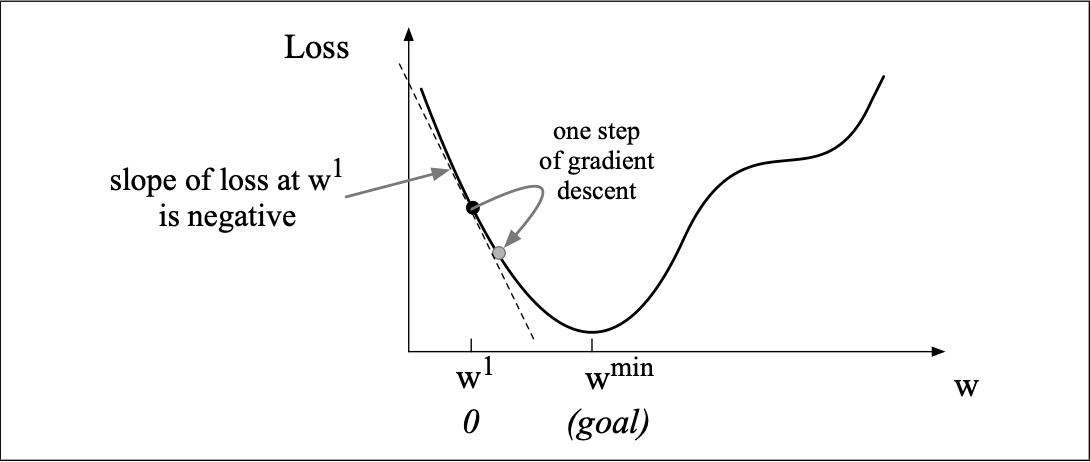
\includegraphics[width=0.5\linewidth]{pic/Klassifikation/MinimumSuche.png}
\caption{\label{pic:MinimumSuche} Iterative Suche nach dem Minimum}
\end{figure}


Basierend auf den Gradientenvektor 
\begin{equation}
\Delta L (f(x;\theta),y) = \begin{bmatrix}  \frac{\delta}{\delta w_{1}} L (f(x;\theta),y) \\ 
 \frac{\delta}{\delta w_{2}} L (f(x;\theta),y) \\ 
. \\ 
. \\ 
. \\ 
  \frac{\delta}{\delta w_{n}} L (f(x;\theta),y) \\ 
   \frac{\delta}{\delta b} L (f(x;\theta),y) \end{bmatrix} \label{Gradientenvektor}
\end{equation}
lassen sich neue Gewichte wie folgt berechnen:
\begin{equation}
\theta_{t+1} = \theta_{t} - \eta \Delta L (f(x;\theta),y),  \label{neue Gewichte}
\end{equation}

wobei $\eta$ die Lernrate entspricht. Diese beschreibt wie schnell den Abhang entlang gefahren wird. Die Wahl von $\eta$ hat einen Einfluss auf die Geschwindigkeit der Suche nach dem Minimum. Ist $\eta$ zu klein gewählt, ist die Laufgeschwindigkeit langsamer und andersrum ist die Laufgeschwindigkeit schneller, wenn $\eta$ groß gewählt ist. Ist jedoch $\eta$ zu groß gesetzt, könnte man das Minimum verpassen. Die Lernrate soll daher optimal gewählt werden, sodass die Laufgeschwindigkeit groß genug ist, um das Minimum schnellstmöglich zu finden und gleichzeitig das System nicht mit unnötig vielen Berechnungen zu belasten.

\begin{figure}[H]
\centering
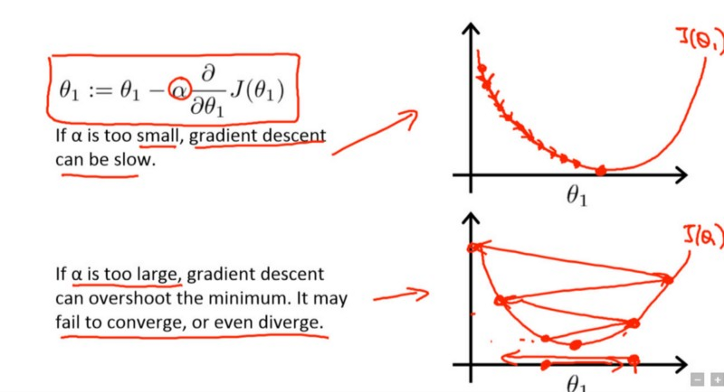
\includegraphics[width=0.5\linewidth]{pic/Klassifikation/Lernrate.png}
\caption{\label{pic:Lernrate} Einfluss der Lernrate auf die Suche nach dem globalen Minimum}
\end{figure}

\subsection{EfficientNet}
\label{EfficientNet}
Die final gewählte Architektur ist ein EfficientNet, dessen Besonderheit gegenüber früheren Neuronalen Netzen es ist, die Parameter der Auflösung (Größe der Eingabebilder), Breite (Anzahl Neuronen je Layer) und Tiefe (Anzahl Layer) des Netzes im optimalen Verhältnis zu skalieren. Die Intuition ist, dass je größer die Auflösung ist, desto breiter und tiefer muss das Netz sein, um dessen Eigenschaften zu repräsentieren, aber eine weitere Verbreiterung und Vertiefung über das Verhältnis hinaus (bei gleichbleibender Auflösung) sinkende Erträge erzielt und somit durch verlangsamtes Training das Gesamtmodell verschlechtert.

Mathematisch ist es ein Optimierungsproblem mit den Parametern Tiefe $d = \alpha^\oslash$, Breite $w = \beta^\oslash$, Auflösung $r = \gamma^\oslash$, sodass $\alpha.\beta^2.\gamma^2 \approx 2$, wobei $\alpha,\beta,\gamma$ mit einem Grid Search Algorithmus bestimmt werden. Die Floating Point Operations Per Second (FLOPS) sind durch $(\alpha.\beta^2.\gamma^2)^\oslash$ berechenbar. Da $\alpha.\beta^2.\gamma^2$ etwa 2 ist, erhöht sich für jedes weitere $\oslash$ die Anzahl der FLOPS um $2^\oslash$. Wenn $\oslash = 1$ ergibt eine GridSearch mit $\alpha.\beta^2.\gamma^2 \approx 2$ die Werte $\alpha = 1.2, \beta = 1.1, \gamma = 1.15$. Dies ist das EfficientNet-B0 Modell. Für die Modelle B1-B7 werden die eben genannten Werte für $\alpha, \beta, \gamma$ nur noch skaliert.

\begin{figure}[H]
\centering
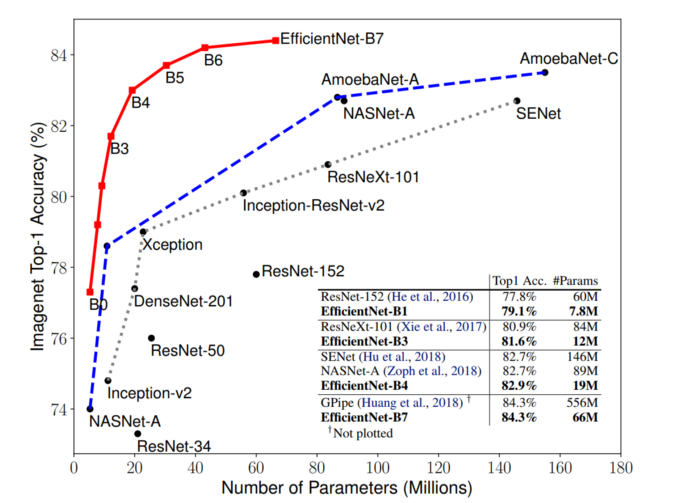
\includegraphics[width=0.5\textwidth]{./pic/Klassifikation/EfficientNetPerformance.png}
\caption{Anzahl Parameter und Performance im Vergleich. \textit{Quelle}: \cite{22}}
\end{figure}

\section{Umsetzung}

Die Umsetzung der Klassifikation geschieht über die Nutzung eines in PyTorch vorimplementierten EfficientNet \cite{22}. Die gewählte Größe unseres EfficientNet ist das größte welches zum Zeitpunkt des Projektes zur Verfügung steht - B7.  Das Netz arbeitet hierbei auf Bildern der Maße 448x448 und ist somit den 509x496 der OCTs der Uniklinik am nächsten. Um die notwendige Auflösung zu erhalten müssen die Ränder der Bilder also beschnitten werden. Dies geschieht ohne erwartete Verluste, da das uns vermittelte Expertenwissen darauf hindeutet dass Ödeme, insbesondere zu behandelnde Ödeme, sich meist zentral auf den Querschnitten befinden.

Desweiteren werden die Bilder vor der Eingabe transformiert, um Kontraste klarer werden zu lassen. Dies passiert indem zunächst die Mittelwerte und Standartabweichungen der RGB Werte des gesamten Datensatzes ermittelt und die RGB Werte der Bilder damit anschließend normalisiert werden, wie zu sehen in Abbildung \ref{pic:Norm}.

Das EfficientNet-B7 wurde auf dem ImageNet Datensatz vortrainiert, welches aus 14.197.122 hochauflösenden Bildern mit 27 Klassen besteht. Dies dient als gute Baseline um Formen und Kanten auf Bildern zu erkennen.

\begin{figure}[H]
\centering
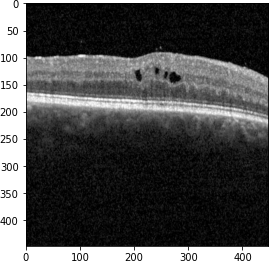
\includegraphics[width=0.25\textwidth]{./pic/Klassifikation/regular_image.png}\hspace{0.5cm}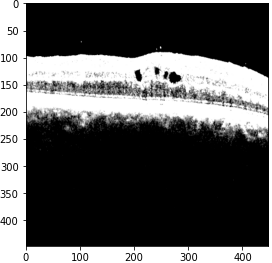
\includegraphics[width=0.25\textwidth]{./pic/Klassifikation/normalized_image.png}
\caption{\label{pic:Norm}Normalisierung der RGB Werte}
\end{figure}

Das letzte Neuron des EfficientNet, welches zur Klassifikation dient, wird mit einem Logistischen Regression Neuron ersetzt, welches ebenfalls auf den Features des vorletzten Layers trainiert wird, um letztlich in die Klassen Ödem und kein Ödem zu klassifizieren. Um die Bedingungen für die Logistische Regression zu optimieren, werden die Features außerdem vor deren Eingabe skaliert.

\begin{figure}[H]
\centering
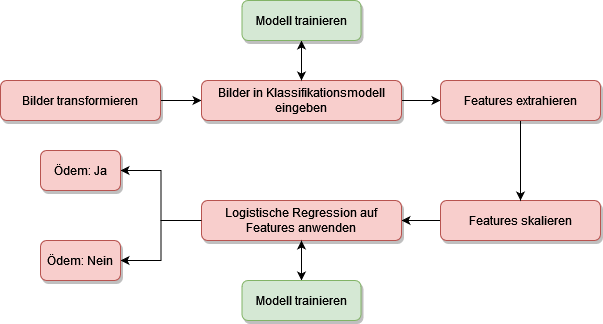
\includegraphics[width=0.7\textwidth]{./pic/Klassifikation/flowchart.png}
\caption{Architektur des Prototypen. - \textit{erstellt mit}: \cite{23}}
\end{figure}

\section{Evaluation}

Zur Evaluation werden zusätzlich zu den extrahierten Features durch das Basis EfficientNet auch die Features nach jeder Finetuning Epoche auf den Trainings- und Testdaten gespeichert, diese mit unterschiedlichen Skalierern skaliert und die jeweiligen skalierten Trainingsfeatures für das Training der Logistischen Regression mit variierenden Hyperparametern verwendet, um dessen Ergebnisse dann mit dem identischen Verfahren auf den Testfeatures zu evaluieren (Abbildung \ref{tab:res1} und \ref{tab:res2}).

Die Evaluation geschieht dann auf den Metriken (Abbildung \ref{tab:Metr}) der Sensitivity und Specificity, mit einer höheren Wertlegung auf die Sensitivity, da die Klassifikation ein Vorfilter für die Segmentierung darstellen sollte, sowie die gesamte Makulaerkennung einen Vorfilter für die Experteneinschätzung der Ärzte, wobei es bei einem Vorfilter viel kritischer ist einen kranken Patienten als gesund zu deklarieren als umgekehrt.

Desweiteren ist es notwendig einen Threshold für die Klassifikation der Logistischen Regression zu bestimmen, tendierend wieder zum Sensitivity bevorzugenden Wertebereich $[0, 0.5]$.

\begin{figure}[H]
\centering
\begin{tabular}{cc c cc}
\multicolumn{2}{c}{\textbf{Treffsicherheit (Klassen)}} && \multicolumn{2}{c}{\textbf{Relevanz (Positive)}} \\
sensitivity: & $\frac{tp}{tp+fn}$ && precision: & $\frac{tp}{tp+fp}$ \\
specificity: & $\frac{tn}{fp+tn}$ && recall: & $\frac{tp}{tp+fn}$
\end{tabular} \\\vspace{0.1cm}
{\footnotesize tp = True Positives, tn = True Negatives, fp = False Positives, fn = False Negatives}
\caption{\label{tab:Metr}Bei der Evaluation verwendete Metriken}
\end{figure}

\begin{figure}[H]
\centering
\begin{tabular}{c|c|c|c|c}
\textbf{epoch} & \textbf{threshold} & \textbf{sensitivity} & \textbf{specificity} & \textbf{sensitivity+specificity} \\\hline\hline
0 & 0.3 & 0.88 & 0.80 & 1.68 \\
0 & 0.4 & 0.83 & 0.85 & 1.68 \\
1 & 0.2 & 0.89 & 0.81 & 1.71 \\
1 & 0.3 & 0.86 & 0.86 & 1.72 \\
1 & 0.4 & 0.85 & 0.88 & 1.73 \\
1 & 0.5 & 0.83 & 0.90 & 1.73 \\
1 & 0.6 & 0.81 & 0.91 & 1.72 \\
\textcolor{red}{2} & \textcolor{red}{0.2} & \textcolor{red}{0.91} & \textcolor{red}{0.83} & \textcolor{red}{1.74} \\
2 & 0.3 & 0.88 & 0.87 & 1.75 \\
2 & 0.4 & 0.86 & 0.89 & 1.75 \\
2 & 0.5 & 0.84 & 0.90 & 1.74 \\
2 & 0.6 & 0.82 & 0.91 & 1.72 \\
3 & 0.3 & 0.86 & 0.86 & 1.72 \\
3 & 0.4 & 0.84 & 0.88 & 1.72 \\
3 & 0.5 & 0.82 & 0.90 & 1.71 \\
4 & 0.2 & 0.90 & 0.84 & 1.73 \\
4 & 0.3 & 0.87 & 0.88 & 1.75 \\
4 & 0.4 & 0.85 & 0.89 & 1.74 \\
4 & 0.5 & 0.82 & 0.91 & 1.73 \\
5 & 0.2 & 0.87 & 0.81 & 1.68 \\
5 & 0.3 & 0.83 & 0.87 & 1.70 \\
6 & 0.2 & 0.85 & 0.84 & 1.69 \\
6 & 0.3 & 0.82 & 0.89 & 1.71 \\
7 & 0.2 & 0.82 & 0.87 & 1.69 \\
8 & 0.2 & 0.83 & 0.83 & 1.66
\end{tabular}
\caption{\label{tab:res1}Klassifikatoren mit sowohl Sensitivity als auch Specificity >= 0.8, \\ Addition der Metriken nur zur Erleichterung eines Vergleichs, der gewählte Favorit in rot}
\end{figure}

\begin{figure}[H]
\begin{tabular}{c|c|c|c|c|c|c}
\textbf{epoch} & \textbf{scaler} & \textbf{solver} & \textbf{threshold} & \textbf{sensitivity} & \textbf{specificity} & \textbf{sensitivity+specificity} \\\hline\hline
1 & StandartScaler & newton-cg & 0.2 & 0.90 & 0.81 & 1.71 \\
1 & StandartScaler & lbfgs & 0.2 & 0.90 & 0.82 & 1.72 \\
1 & StandartScaler & liblinear & 0.2 & 0.90 & 0.82 & 1.72 \\
1 & RobustScaler & lbfgs & 0.2 & 0.91 & 0.80 & 1.71 \\
2 & StandartScaler & newton-cg & 0.2 & 0.91 & 0.82 & 1.74 \\
2 & StandartScaler & lbfgs & 0.2 & 0.91 & 0.82 & 1.74 \\
2 & StandartScaler & liblinear & 0.2 & 0.91 & 0.82 & 1.74 \\
2 & StandartScaler & sag & 0.2 & 0.91 & 0.82 & 1.73 \\
2 & StandartScaler & saga & 0.2 & 0.91 & 0.82 & 1.73 \\
2 & RobustScaler & newton-cg & 0.2 & 0.92 & 0.81 & 1.73 \\
\textcolor{red}{2} & \textcolor{red}{RobustScaler} & \textcolor{red}{liblinear} & \textcolor{red}{0.2} & \textcolor{red}{0.93} & \textcolor{red}{0.82} & \textcolor{red}{1.75} \\
2 & RobustScaler & liblinear & 0.3 & 0.91 & 0.85 & 1.76 \\
3 & StandartScaler & newton-cg & 0.2 & 0.90 & 0.80 & 1.71 \\
3 & StandartScaler & lbfgs & 0.2 & 0.90 & 0.80 & 1.71 \\
3 & StandartScaler & liblinear & 0.2 & 0.90 & 0.80 & 1.71
\end{tabular}
\caption{\label{tab:res2}
Variierende Skalierer und Solver für die Logistische Regression, Klassifikatoren mit Sensitivity >= 0.9 und Specificity >= 0.8, Addition der Metriken nur zur Erleichterung eines Vergleichs, unser gewählter Favorit in rot}
\end{figure}

Die Performance des Favoriten mit Skalierer und angepasstem Solver werden nun noch in Hinsicht der Precision und Recall (=Sensitivity) Werte analysiert (siehe Abbildung \ref{pic:Eval}).

\begin{figure}[H]
\label{pic:Eval}
\centering
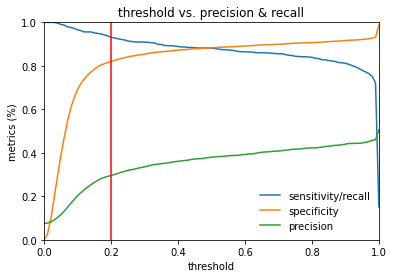
\includegraphics[width=0.7\textwidth]{./pic/Klassifikation/eval.png}
\caption{Performance nach Threshold}
\end{figure}

Wie man sehen kann flacht das Wachstum der Specificity und Precision bei etwa einem Threshold von 0.2 ab, während Sensitity/Recall stetig abnimmt. Dies bestätigt erneut den gewählten Threshold, um Sensitivity/Recall so hoch wie möglich zu halten, ohne alles willkürlich als positiv zu deklarieren.

\textbf{Sensitivity}: 0.98, \textbf{Specificity}: 0.82; \textbf{Precision}: 0.3, \textbf{Recall}: 0.98

Ein Precision Wert von 0.3 wirkt besonders gering, ist jedoch bei einem Klassenunverhältnis wie diesem zu erwarten, da sehr viele negative Bilder die Chance haben, fälschlicherweise als positiv deklariert zu werden und die Precision das Verhältnis an wirklich positiven gegenüber wirklich negativen der als positiv vorhergesagten Bilder beschreibt.




% ---------------------------------------------------------------------------------------------------------
\chapter{Segmentierung}
% ----------------------------
%allgemeines zu Sinn und Zweck der Segmentierung
Neben der binären Klassifikation von Ödem oder kein Ödem sind weitere Fragestellungen von Interesse. Insgesamt sollen weitere Aspekte 
untersucht werden, welche aufeinander aufbauen (s. Abb. \ref{fig:ziel_segmentierung}).

Feingranularer als die binäre Klassifikation von Ödemen, ist die Erkennung individueller Ödeme. Somit können sowohl die Anzahl von Ödemen auf einem Bild bestimmt, als auch später die Erhebung weiterer Kennzahlen pro Ödem erhoben und kontrolliert werden.
Hierzu zählt die Berechnung der Größe eines Ödems. Neben der Lage der Flüssigkeitsansammlung kann deren Größe Einfluss auf den Grad der Beeinträchtigung des Patienten nehmen. Somit ist im Rahmen der Verlaufskontrolle einer Therapie das dritte Ziel begründet: Durch Erhebung der Größe von Ödemen eines Patienten zu jedem OCT-Scan kann eine Größenveränderung ein Indikator für den Erfolg der Therapie darstellen.\newline
\begin{figure}[ht!]
\centering
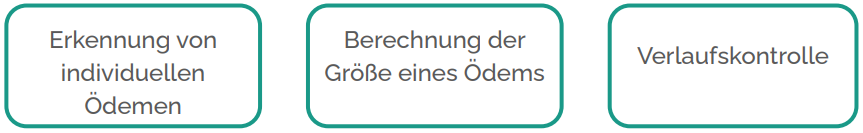
\includegraphics[width=0.7\linewidth]{./pic/Segmentierung/ziel_segmentierung.png}
\caption{\label{fig:ziel_segmentierung}Die drei Ziele, welche im Rahmen der Segmentierung erreicht werden sollen.}
\end{figure}

Diese Ziele können nicht mit der binären Klassifikation erreicht werden. Das folgende Kapitel beschäftigt sich mit dem Verfahren der Instanzsegmentierung, welches für die Erkennung und Ausmessung einzelner Objekte in Bildern entwickelt wurde. 



% ----------------------------
\section{Architektur}
% ----------------------------

CNNs, bereits im Unterabschnitt \ref{CNN} vorgestellt, dienen als Grundlage für die Entwicklung effizienterer Architekturen im Bereich der Bildsegmentierung: insbesondere in der Objekterkennung, Semantischen Segmentierung  sowie Instanzsegmentierung.  

\begin{figure}[H]
\centering
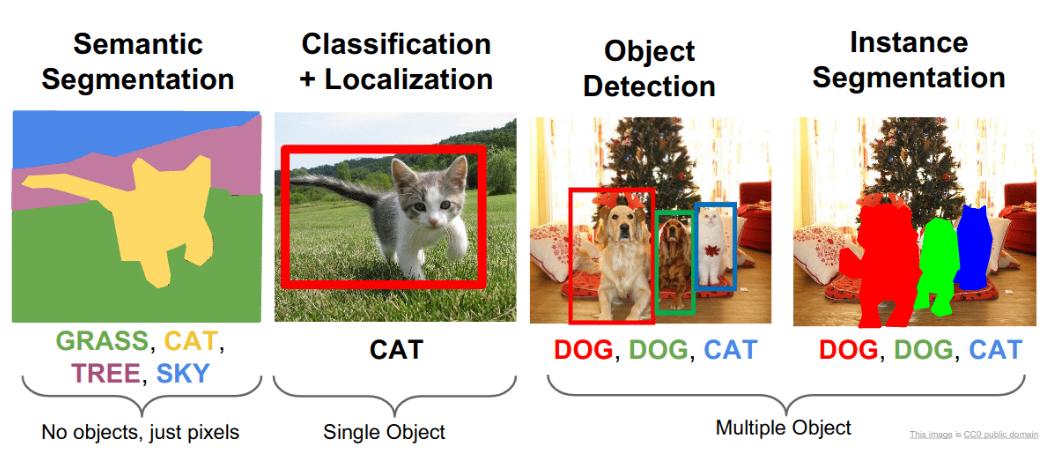
\includegraphics[width=0.7\linewidth]{pic/Segmentierung/segmentation_catsndogs.png}
\caption{\label{pic:catsndogs} Arten der Segmentierung}
\end{figure}


Die erste Architektur der Objekterkennung lässt sich auf Region Based CNN, auch R-CNN genannt, zurückführen. Im Vergleich zu CNNs klassifiziert R-CNN nicht das gesamte Bild, sondern jedes einzelne Objekt in einem Bild. Dabei wird jedes Objekt mit einer Bounding Box versehen und anschließend einzeln in das CNN zur Feature Extraction und Klassifizierung weitergegeben. Die Suche nach sogenannten Region Proposals, also Regionen, wo Objekte enthalten könnten, läuft im R-CNN mit der Selektiven Suche. Da die Suche nach Region Proposals mit der Selektiven Suche sehr zeitaufwendig und ineffizient ist, wurde sie in den folgenden Jahren im Faster R-CNN durch ein Region Proposal Netzwerk (RPN) ersetzt. 

Semantische Segmentierungsverfahren wie z.B. das Fully Convolutional Netzwerk (FCN) sind für das Maskieren der Objekte auf Pixel Ebene verantwortlich. Eine Einschränkung in der Semantischen Segmentierung besteht darin, dass Objekte derselben Klasse in einem Bild nicht voneinander unterschieden werden. Existieren z.B. zwei Katzen in einem Bild, werden alle entsprechende Pixel dem Label Katze zu geordnet und nicht differenziert zwischen Katze 1 und Katze 2.

Die Instanzsegmentierung behebt die Einschränkung der Semantischen Segmentierung. Zudem wird jedes Objekt mit einer Bounding Box lokalisiert. Die Instanzsegmentierung vereint also die Elemente der Objekterkennung mit denen der Semantischen Segmentierung und bietet eine höhere Genauigkeit im Bereich der Bildsegmentierung. 

% ----------------------------
\subsection{Mask R-CNN}
% ----------------------------

Für das Projekt wurde das Mask R-CNN als Architektur der Instanzsegmentierung gewählt, welches Faster R-CNN aus der Objekterkennung mit dem Fully Convolutional Netwerk (FCN) aus der Semantischen Segmentierung in seiner Architektur vereint. Genauer gesagt erweitert das Mask R-CNN die Architektur der Faster R-CNN um den sogenannten mask branch (s. Abb. \ref{pic:mask_rcnn}), um das Maskieren der Objekte zu ermöglichen. 

\begin{figure}[H]
\makebox[\linewidth]{%
  \begin{tabular}{cc}
    Faster R-CNN Architektur & Mask R-CNN Architektur\\
    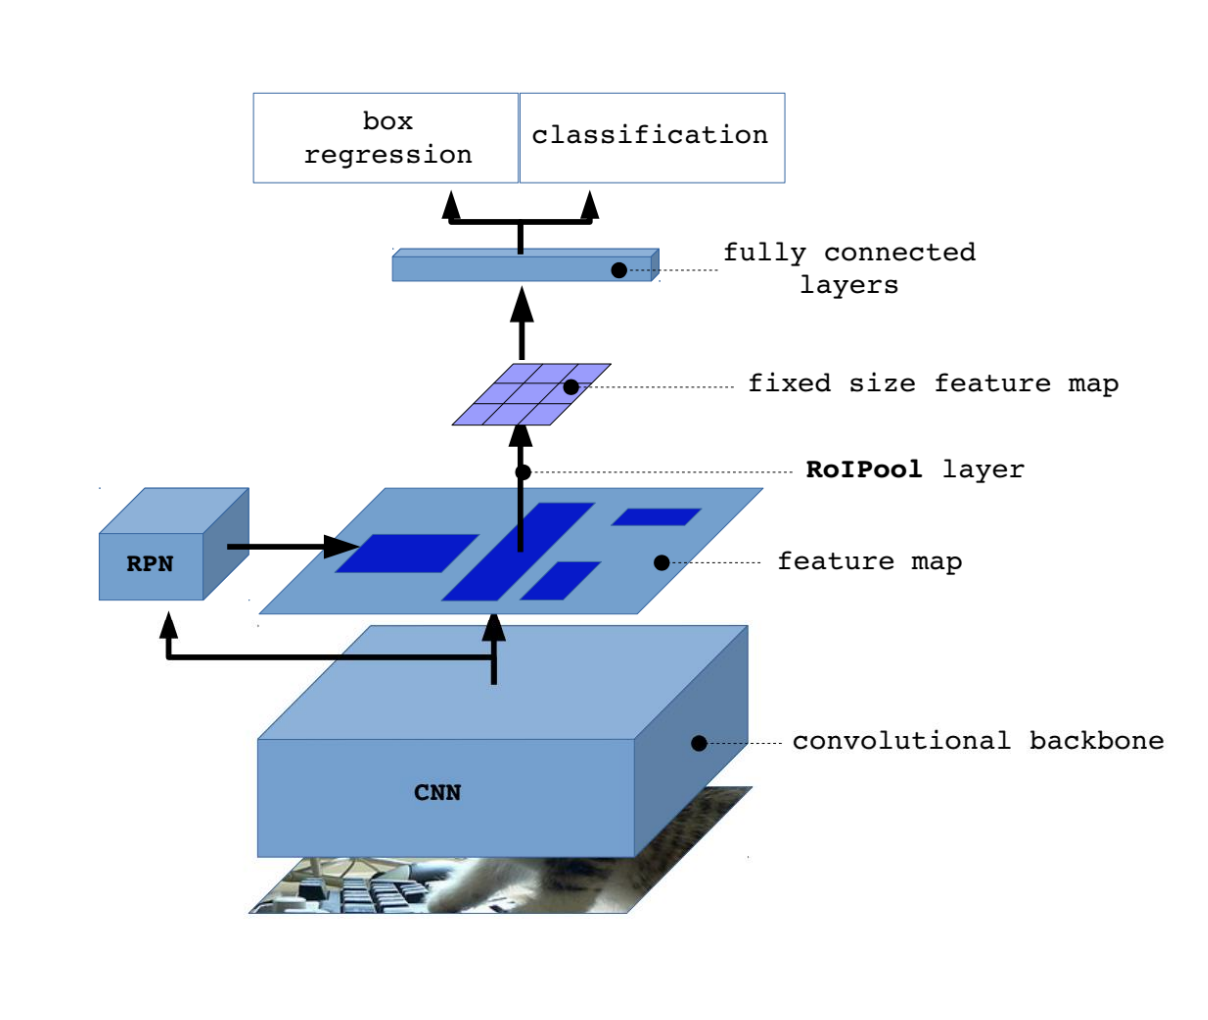
\includegraphics[width=0.4\linewidth]{pic/Segmentierung/faster_rcnn.png}&
    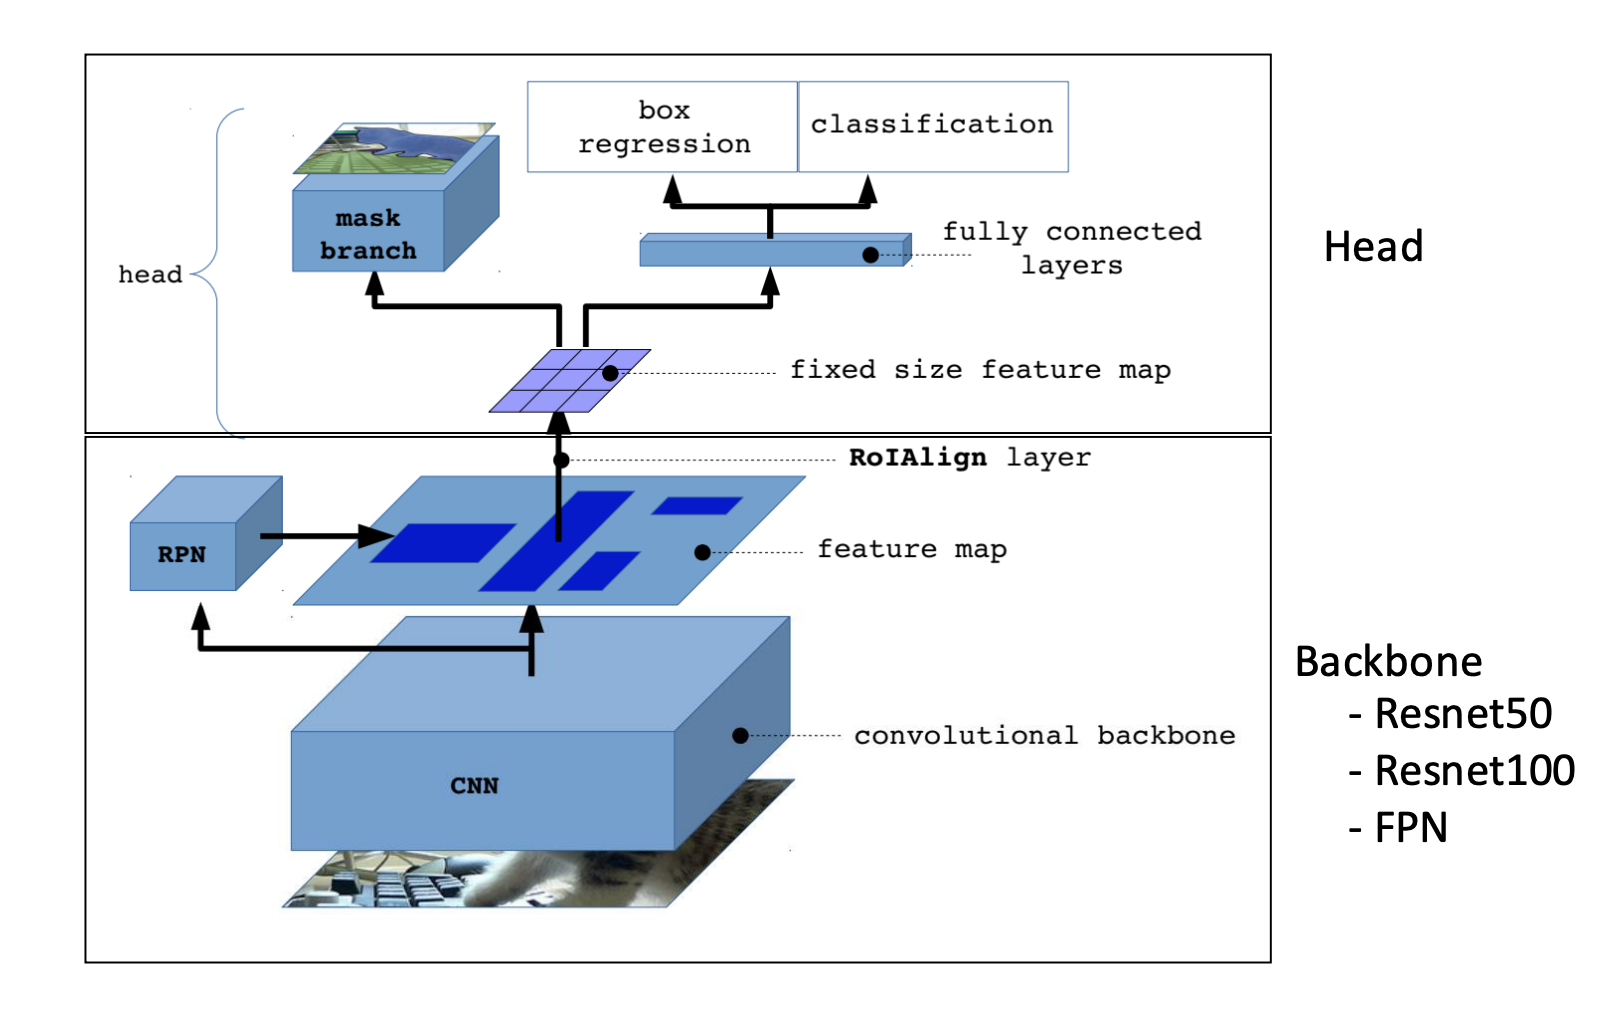
\includegraphics[width=0.5\linewidth]{pic/Segmentierung/mask_rcnn.png}\\
  \end{tabular}%
}
 \caption{Mask R-CNN als Erweiterung des Faster R-CNNs um den Mask Branch}
  \label{pic:mask_rcnn}
\end{figure}

Mask R-CNN ist, wie in \cite{7} und \cite{8} erklärt, ein zweistufiges Verfahren. Die erste Stufe nennt sich Backbone und die zweite heißt Head. Das Backbone enthält ein CNN und ein RPN, mit denen eine Feature Map mit Region Proposals erzeugt wird. Als Backbone Architektur verwendet Mask R-CNN oft ein Resnet50, Resnet100 oder Future Pyramid Netzwerk(FPN). Der Head ist für die Klassifikation und das Maskieren der Objekte verantwortlich.

Um das Konzept des Mask R-CNNs zu verstehen, wird das Vorwissen über CNNs vorausgesetzt, daneben ist das Wissen über das Region Proposal Netzwerk und Fully Convolutional Network von Bedeutung, da sie die wesentlichen Konzepte im Mask R-CNN sind. In den nächsten Unterabschnitten wird auf das Region Proposal Netzwerk (RPN) zur Suche nach Region Proposals (in \ref{subsec:RPN}) und Fully Convolutional Netzwerk (FCN) zum Maskieren der Objekte auf Pixel Ebene (in \ref{subsec:FCN}), eingegangen. Dabei wurde der Unterabschnitt RPN mithilfe von den Quellen \cite{9}, \cite{10} und \cite{11}) verfasst und der Unterabschnitt FCN in Anlehnung an den Arbeiten \cite{12}, \cite{13}, \cite{17}, \cite{18}, \cite{19}, \cite{20} und \cite{21}) erstellt.


% ----------------------------
\subsection{Region Proposal Netzwerk (RPN)} \label{subsec:RPN}
% ----------------------------
Die deutliche Verbesserung in der Laufzeit des Mask R-CNNs im Vergleich zum R-CNN lässt sich vor allem auf das Ersetzen der Selektiven Suche durch das zum Algorithmus integriertes RPN zurückführen. 

Wie ein CNN die Klassifizierung aus der Feature Map lernt, lernt auch RPN Region Proposals aus der Feature Map, dies erfolgt im Wesentlichen in 3 Schritten:

\begin{enumerate}
\item Generiere Anker-Punkte.
\item Generiere Anker-Boxen.
\item Klassifiziere Anker-Boxen in die Klassen Vordergrund (positiv) oder Hintergrund (negativ) und lerne die Abweichungen zwischen der positiven Anker-Boxen und der  Grundwahrheitsboxen.
\end{enumerate}

\begin{figure}[H]
\centering
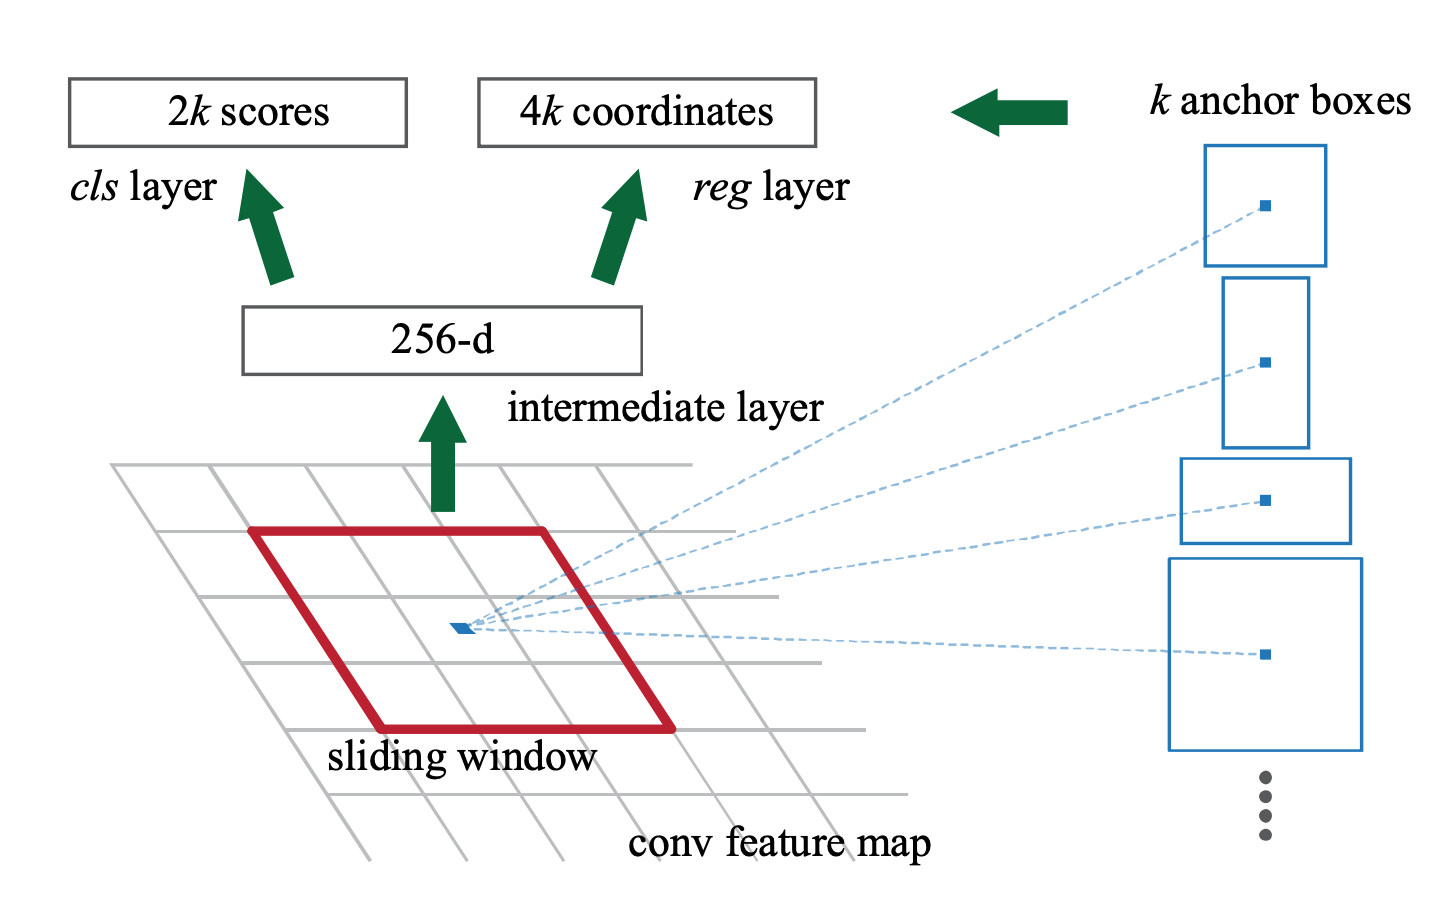
\includegraphics[width=0.5\linewidth]{pic/Segmentierung/RPN_architektur.png}
\caption{\label{pic:rpn} RPN Architektur}
\end{figure}

Die Anker-Punkte werden mit einem gleitenden Fenster (Sliding Window), wie in der obigen Abbildung \ref{pic:rpn} gezeigt, generiert. Die Anzahl der zu generierenden Anker-Punkte hängt von dem Stride des gleitenden Fensters ab, wobei der Stride von der Backbone Architektur entschieden wird. 
\begin{figure}[H]
\centering
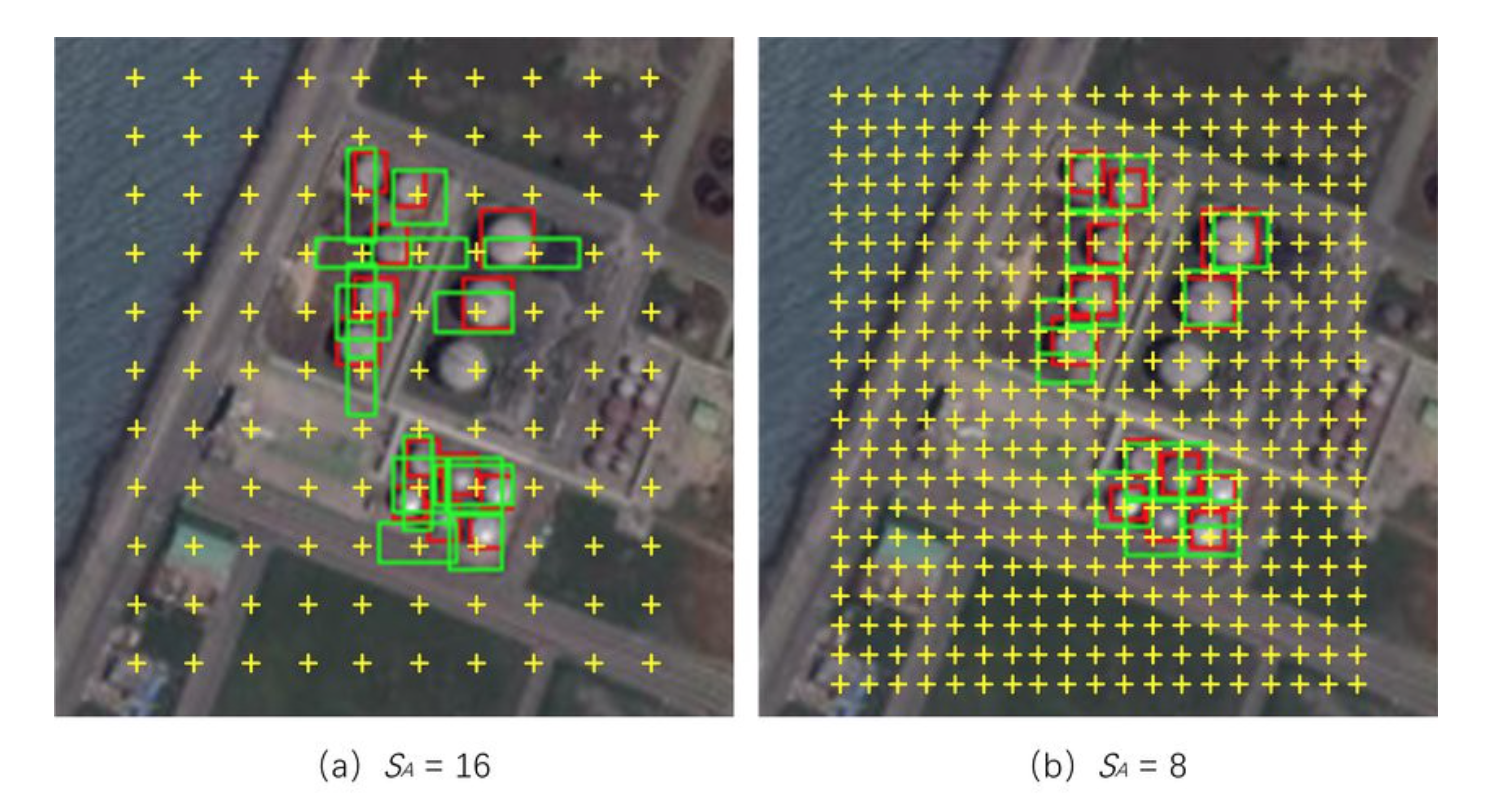
\includegraphics[width=0.7\linewidth]{pic/Segmentierung/Segmentierungsergebnisse/Anker-Punkte.png}
\caption{\label{pic:Anker-Punkte} Anzahl der generierten Anker-Punkte abhängig von dem Stride }
\end{figure}

Nun werden Anker-Boxen verschiedener Größen und Seitenverhältnisse definiert und auf jeden Anker-Punkt gelegt. Im dem ursprünglichen Paper \cite{9} definieren Shaoqing Ren et al. 3 verschiedene Größen: 128$\times$128, 256$\times$256, 512$\times$512 und 3 verschiedene Seitenverhältnisse: 1:1, 1:2, 2:1. Es gibt Anker-Boxen, die Objekte enthalten und Anker-Boxen, die keine Objekte umfassen. Ziel des nächsten Schrittes ist es, Anker-Boxen entsprechend in den Klassen Vordergrund (positiven) und Hintergrund (negativen) zu klassifizieren, dies erfolgt in der Classification Layer (cls layer, s. Abb.\ref{pic:rpn}) und gleichzeitig die Abweichungen zwischen der positiv klassifizierten Anker-Boxen und der Grundwahrheitsboxen in der Regression Layer (reg layer, s. Abb.\ref{pic:rpn}) zu berechnen.

Für die Klassifizierung der Anker-Boxen wird die Intersection over Union (IoU) als Entscheidungsgröße verwendet. 
\begin{Definition}[IoU]
IoU ist eine relative Maßzahl, welche die Stärke der Überschneidung zwischen einer Anker-Box und einer Grundwahrheitsbox beschreibt. Sie ist wie folgt definiert:
\begin{equation}
IoU = \frac{\textrm{Area of Overlap}}{\textrm{Area of Union}}. \label{IoU}  
\end{equation}
\end{Definition}
Die Entscheidungsregel für eine positive Anker-Box auf Grundlage der $IoU$ lautet: Eine Anker-Box mit der höchsten IoU oder mit einer IoU > 0.7 wird positiv klassiziert. Demzufolge erhält jede Anker-Box mit einer IoU < 0.3 ein negatives Label.

Gleichzeitig werden die Koordinaten $x$, $y$, $w$ und $h$ der positiven Anker-Boxen und Grundwahrheitsboxen ermittelt und anschließend deren Differenzen der Koordinaten berechnet. Dabei geben $(x,y)$ die Koordinaten des Mittelpunktes einer Box an und $w$ und $h$ entsprechen jeweils die Breite und Höhe der Box. Die Differenzen werden in der Regression Layer gelernt und minimiert. um die Prognosen der Region Proposals mit Bouding Boxen zu optimieren.

% ----------------------------
\subsection{Fully Convolutional Netzwek (FCN)} \label{subsec:FCN}
% ----------------------------
FCN ist ein Konzept der Semantischen Segmentierung und ermöglicht das Maskieren von Objekten auf Pixel Ebene im Mask R-CNN. FCN lässt sich unterteilen in zwei Phasen: Convolution Netzwerk und Deconvolution Netwerk. 

\begin{figure}[H]
\centering
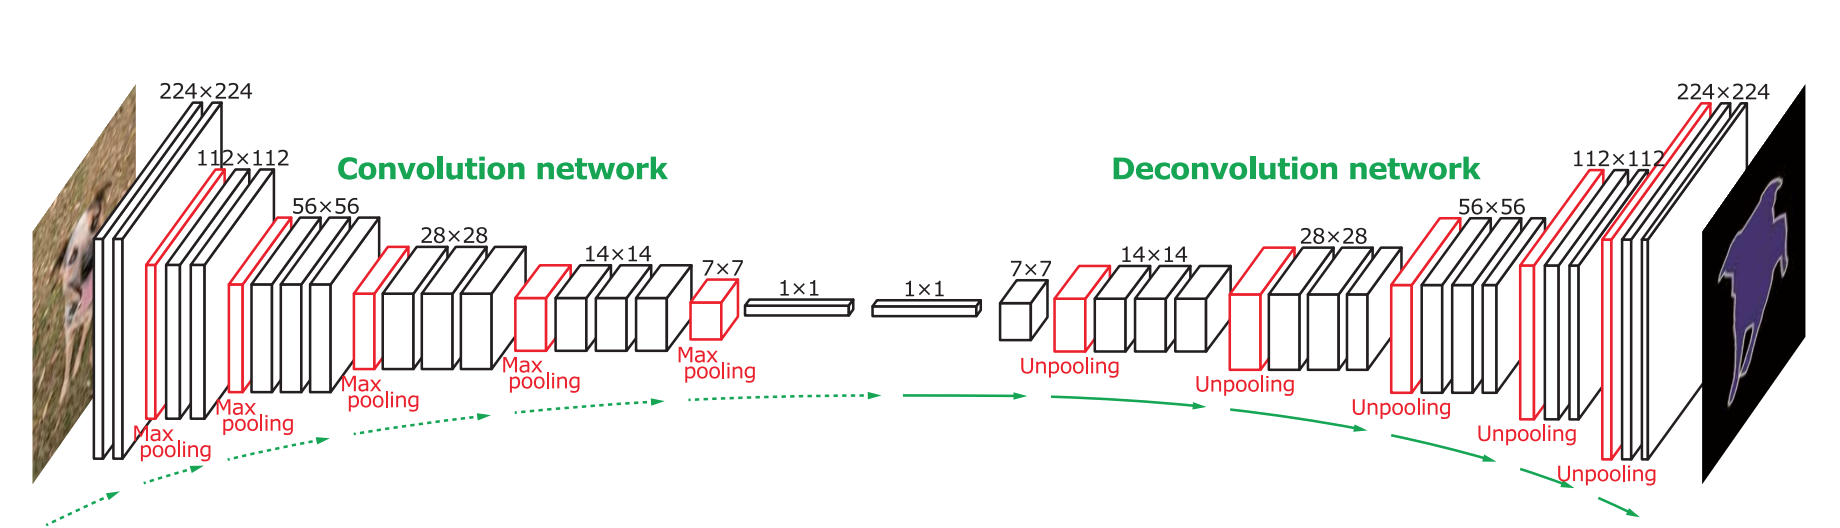
\includegraphics[width=\textwidth]{pic/Segmentierung/ArchitekturFCN.png}
\caption{\label{pic:fcn} Architektur FCN (konkret: VGG-16 Netz)}
\end{figure}

In der ersten Phase wird die räumliche Auflösung des Bildes verkleinert, es wird eine Feature Map erzeugt mit nur wesentlichen Informationen, die das effiziente Lernen von Features zur Klassifizierung auf Pixel Ebene unterstützt. Durch Convolution und Pooling Operationen gehen jedoch die räumlichen Informationen verloren, was das Übertragen der klassifizierten Pixel auf das ursprüngliche Bild Schwierigkeiten bereiten könnte. Diese Schwierigkeit wird in der zweiten Phase im Deconvolution Network mit Unpooling und Transposed Convolution Operationen behoben.


\subsubsection{Convolution Network}
Das Convolution Network ist ähnlich wie das bereits in \ref{CNN} vorgestelltes CNN, es besitzt ebenfalls Convolution Layers, als auch Pooling Layers zum Extrahieren und Lernen von Features. Der einzige Unterschied liegt darin, dass das Convolution Network die Fully Connected Layer im CNN durch eine 1$\times$1 Convolutional Layer ersetzt.  Eine 1$\times$1 Convolutional Layer ist eine 2$d$-Convolution mit einem 1$\times$1$\times$$d$ Kernel, wobei $d$ die Tiefe des Tensor (Input-Matrix) entspricht. Mit dieser Änderung liefert das Convolution Network ein Feature Vektor für jeden Pixel, anstatt ein Feature Vektor für das gesamte Bild wie im CNN. Damit ist die Klassifikation auf Pixel Ebene möglich. Für jedes Objekt wird ein Heatmap geneniert, indem jedes Pixel mit einer Farbintensität gekennzeichnet ist, die die Wahrscheinlichkeit der Anwesenheit des Objektes repräsentiert.


\begin{figure}[H]
\centering
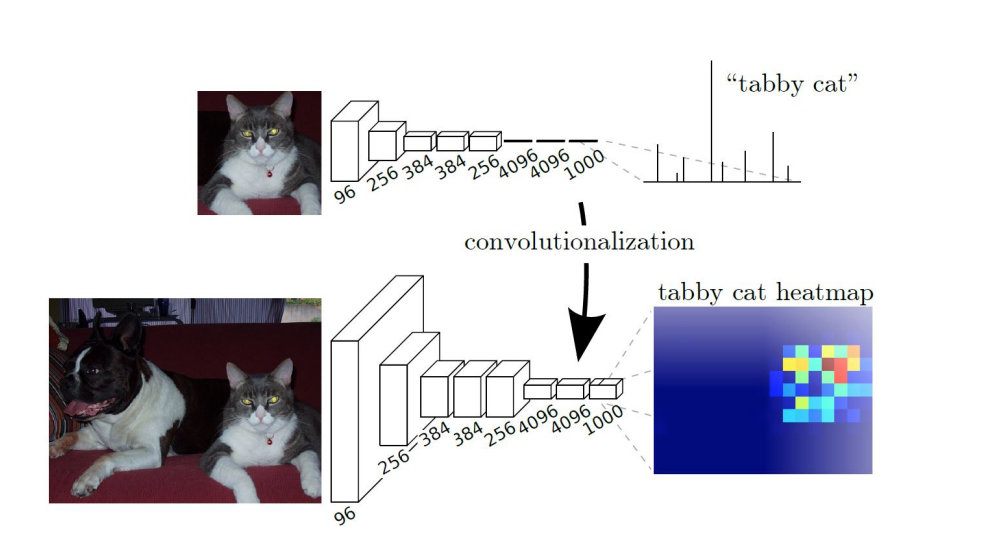
\includegraphics[width=0.8\linewidth]{pic/Segmentierung/Klassifikation_Pixelebene.png}
\caption{\label{pic:class_per_pixel} Klassifikation auf Bildebene vs. Pixelebene}
\end{figure}

\subsubsection{Deconvolution Network}
In dieser Phase geht es darum die geringe Auflösung auf die ursprüngliche Auflösung hochzuskalieren. Dies erfolgt mit den Umkehroperationen (Unpooling und Transposed Convolution) zu denen des Convolution Networks (Pooling, Convolution).

Es gibt verschiedene Unpooling Möglichkeiten: z.B. Nearest Neighbor, Bed of Nails oder Max Unpooling. Beim Nearest Neighbor wird jeder Wert der Input Matrix in die Output Matrix übernommen und gleich oft in die benachbarten Zellen eingefügt.  Beim Bed of Nails wird jeder Wert der Input Matrix in bestimmten Positionen der Output Matrix übernommen und die restlichen Zellen mit Nullen aufgefüllt.
\begin{figure}[H]
\centering
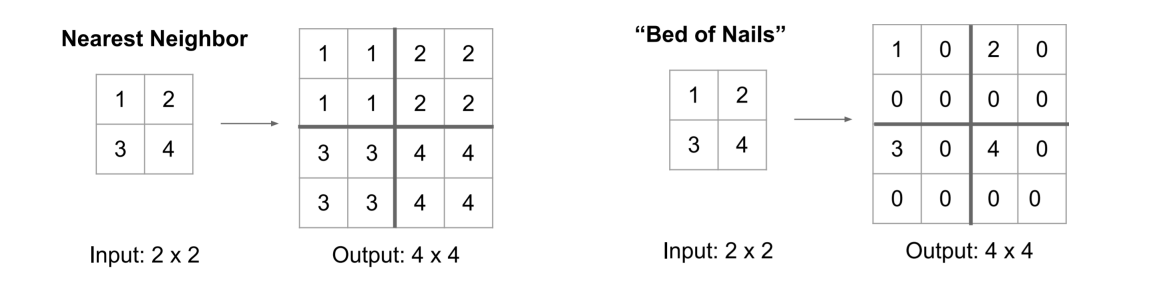
\includegraphics[width=\textwidth]{pic/Segmentierung/NearestNeighbor_BedoofNails.png}
\caption{\label{pic:NN_BoN} Nearest Neighbor und Bed of Nails Unpooling}
\end{figure}
Die Max Unpooling Methode ist die verbesserte Version des Bed of Nails, da die Positionen der Werte in der Output Matrix die Positionen der dazugehörigen Max Pooling Schicht entsprechen. Dies ist möglich wegen der Symmetrie im FCN. 
\begin{figure}[H]
\centering
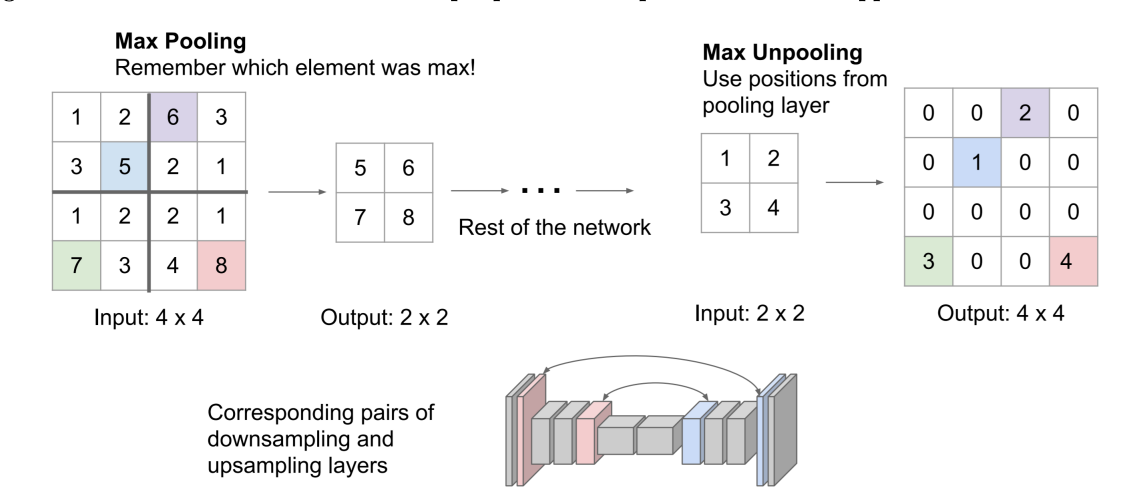
\includegraphics[width=\textwidth]{pic/Segmentierung/MaxUnpooling.png}
\caption{\label{pic:MaxUnpooling} Max Unpooling aufgrund der Symmetrie im FCN}
\end{figure}
Nach dem Unpooling ist die Größe des urspünglichen Tensors wiederhergestellt, wir sehen aber, dass beispielsweise nach dem Max Unpooling noch viele Pixel noch Nullen aufgefüllt sind. Der Informationsverlust wird im Wesentlichen durch Transposed Convolution Operationen behoben. Dabei Zwischentensoren berechnet als Produkt aus der Kernel Matrix und jedes Wertes aus der Input Matrix. Die Zwischentensoren werden anschließend aufsummiert und ergeben die Output Matrix. Die folgende Abbildung illustriert die beschriebene Rechenoperationen.

\begin{figure}[H]
\centering
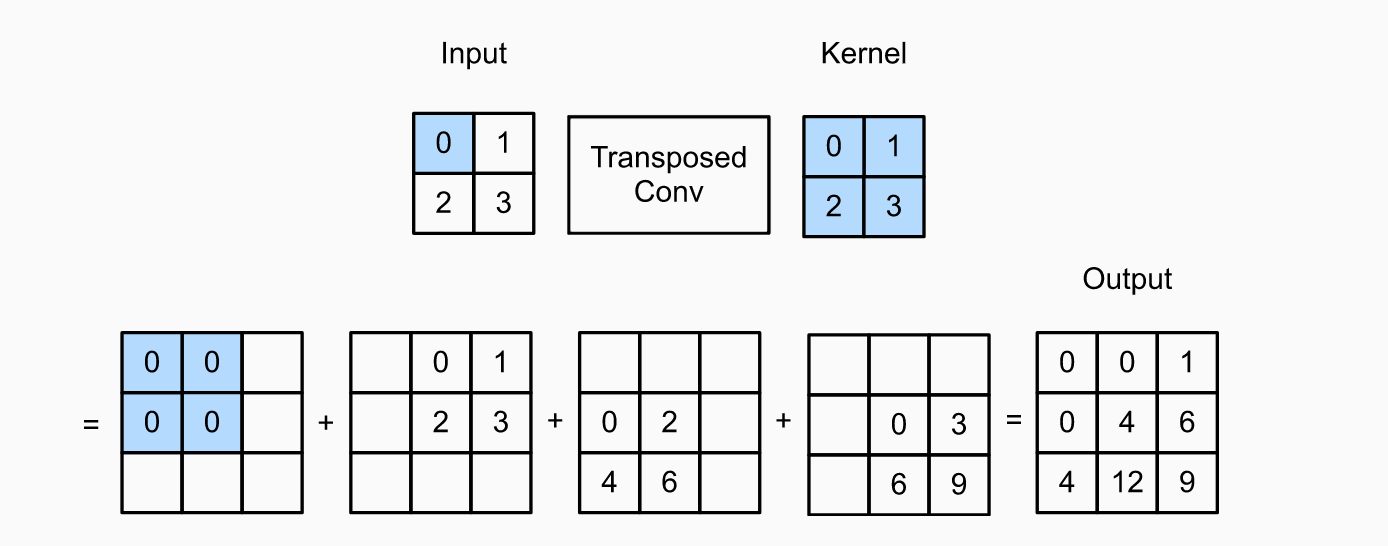
\includegraphics[width=\textwidth]{pic/Segmentierung/TransposedConvolution.png}
\caption{\label{pic:TransposedConvolution} Transposed Convolution mit einem 2x2 Kernel}
\end{figure}

\newpage
\section{Umsetzung}
\subsection{Von den segmentierten Bildern zum trainierten Modell}



Um das Mask R-CNN nicht von Grund auf anlernen zu müssen, wurde ein vortrainiertes Modell als Backbone verwendet. Hierfür wurde das Faster R-CNN ResNet-50 ausgewählt, dass auf dem Common Objects in Context (COCO) Datensatz bereits vortrainiert wurde. 
Der COCO-Datensatz enthält 328 Tausend Bilder mit 80 Objektklassen und 2.5 Millionen gelabelter Segmente. \cite{16}


Der Vorteil der Einbindung des vortrainierten ResNet-50 besteht zum einen darin, dass das ResNet-50 bereits optimiert wurde und somit eine bessere Performance aufweist als ein Modell das von Grund auf erst trainiert werden muss. % hier Beweis/Quelle einfügen
Zum anderen darin, dass mit einer geringen Menge von Bildern gute Resultate im Training erreicht werden können. Da für das Training des Mask R-CNN nur wenige OCT-Bilder zur Verfügung stehen, wirkt sich diese Eigenschaft positiv auf das Ergebnis aus. Die Einbindung des Modells erfolgt über die PyTorch Library.


Nach erfolgreichem Training, können dem Modell nun die Test-Daten übergeben werden, die zur Evaluierung vorgesehen sind.
Auf die Ergebnisse der Evaluierung wird im folgenden Kapitel eingegangen. 

In der folgenden Abbildung \ref{output_mrcnn} ist dargestellt, wie das Ergebnis der Instanzsegmentierung im Output aussieht. 
Auf dem linken Bild ist das korrekt erkannte und gelabelte Ödem mit einer Bounding Box umrahmt. 
Auf der rechten Seite wird das gefundenen Ödem im Bild farblich segmentiert. 

\begin{figure}[H]
\centering
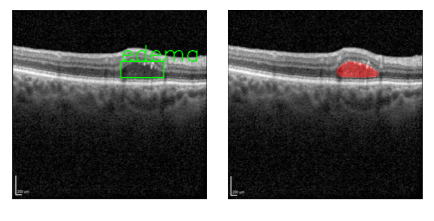
\includegraphics[width=80mm,scale=1.5]{pic/Segmentierung/output_mrcnn.png}
\caption{\label{output_mrcnn}Output Daten des Mask R-CNN (Links: OCT-Bild mit Bounding Box um das gefundene Ödem, Rechts: OCT-Bild mit segmentiertem Ödem)}
\end{figure}



In Abbildung \ref{graph:programmablauf_seg} wird nun aufgezeigt, wie der Programmablauf bei der Erkennung und Segmentierung von Ödemen abläuft.
Dem Segmentierungsmodell wird ein OCT-Bild übergeben. Für das Bild wird durch das Modell eine Vorhersage berechnet, ob Ödeme auf dem Bild vorhanden sind. 
Anschließend werden für alle gefundenen Segmente auf dem Bild die Anzahl der Pixel innerhalb dieser Fläche aufsummiert. 
Abschließend erfolgt dann über das Programm die Ausgabe der Größe des segmentierten Ödems. Die Größenangabe erfolgt hierbei in der Pixelanzahl. 
Wurde kein Ödem auf dem Bild segmentiert, so erfolgt in der Ausgabe eine Größenangabe von 0. 

\begin{figure}[H]
\centering
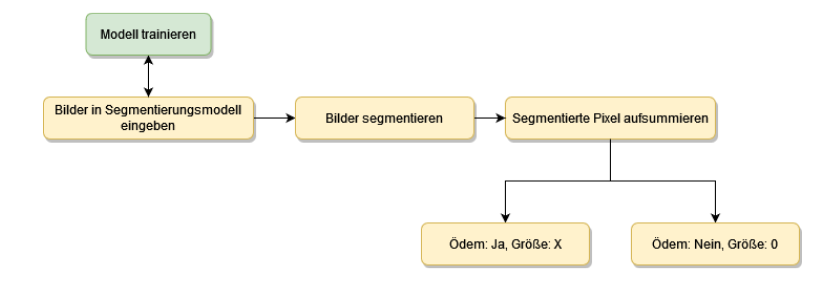
\includegraphics[width=120mm,scale=1.5]{pic/Segmentierung/programmablauf_segmentation.png}
\caption{\label{graph:programmablauf_seg}Programmablauf des Segmentierungsmodells. - \textit{erstellt mit}: \cite{23}}
\end{figure}

\subsection{Erstellen augmentierter Bilder}
Eine Möglichkeit zur Verbesserung der Performanz eines trainierten Modelles ist die Erweiterung des Trainingsdatensatzes \cite{14}. 
Jedoch sind in unserem Anwendungsfall die zur Verfügung stehenden Daten limitiert und es können nicht ohne Weiteres neue Daten erhoben werden.\newline
Um den Trainingsdatensatz ohne die Vermessung weiterer Augen zu erweitern, können Aufnahmen augmentiert werden. Bei der Augmentierung werden die Originalbilder transformiert. Dieselben Transformationen werden dabei an den zugehörigen Masken vorgenommen.\newline
Aufgrund zeitlicher Begrenzung wurde im Rahmen dieses Projektes funktionierender Code zur Datenaugmentierung erstellt, jedoch nicht für das Training verwendet. Als Grundlage für Folgeprojekte wird das Vorgehen in diesem Abschnitt dokumentiert.\newline
Es gibt eine Reihe von Augmentierungsmöglichkeiten. Bei der Auswahl ist es relevant, dass diese auf den konkreten Anwendungsfall passend sind. Daher wurden die Augmentierungsoptionen nach visueller Inspektion aller Patientendaten gewählt.
Insgesamt wurden die folgenden Bildveränderungsmethoden implementiert, welche an einer OCT-Aufnahme in Abb. \ref{fig:segm_augmentiert} visualisiert sind:
\begin{itemize}
    \item Spiegelung an der vertikalen Achse
    \item Drehung um  $\pm$ 15 Grad
    \item Hinzufügen von Rauschen
\end{itemize}

Eine Spiegelung an der vertikalen Achse erweitert den Datensatz auf einfache Weise und ist anatomisch ebenfalls gerechtfertigt, da die Anordnung der Augenschichten durch diese Art der Spiegelung erhalten bleibt. Anders verhält es sich mit der Spiegelung an der horizontalen Achse: Dies ist nicht sinnvoll, da sich ein Makulaödem allgemein über der RPE-Schicht befindet. Bei einer Spiegelung an der horizontalen Achse würde diese lokale Referenz verdreht und die Gefahr eines fehlerhaften Antrainierens der Lage von Ödemen in Relation zu der RPE steigt. Aus dem gleichen Grund sollte eine Drehung der Bilder über 90 Grad vermieden werden. Da die RPE nicht perfekt horizontal sondern in manchen Fällen verkrümmt wirkt, wurde eine Drehung von  $\pm$15 Grad festgelegt. Eine Mögliche Erweiterung wäre eine zufällige Auswahl eines Drehungswinkels im Bereich von $\pm$ 15 Grad um systematische Effekte zu unterdrücken. Da die Augenschichten bei Patienten ungleich sind und eher selten perfekt horizontal im Bild liegen, ist von einem guten Ergebnis auch bei festem Drehwinkel auszugehen. Darüber hinaus besteht durch eine Drehung der Bilder die Möglichkeit, dass antrainierte vertikale Kanten von Segmenten verschwinden und eine dem original nähere Randerkennung erreicht wird. Aufgrund verschiedener Einflussfaktoren wie Alter des Patienten oder weitere Augenerkrankungen werden OCT Bilder verrauschter als bei anderen Patienten. Um die Performanz bei solchen Bildern zu verbessern, wird Gausssches Rauschen auf die Originalbilder, nicht aber auf die Masken hinzugefügt. Die normalverteilten Rauschwerte mit Mittelwert 0 und Standardabweichung 30 werden auf die Pixelwerte addiert. Die resultierenden Pixelwerte werden dabei auf den zugelassenen Bereich von 0 bis 255 begrenzt.
\begin{figure}[h]
\centering
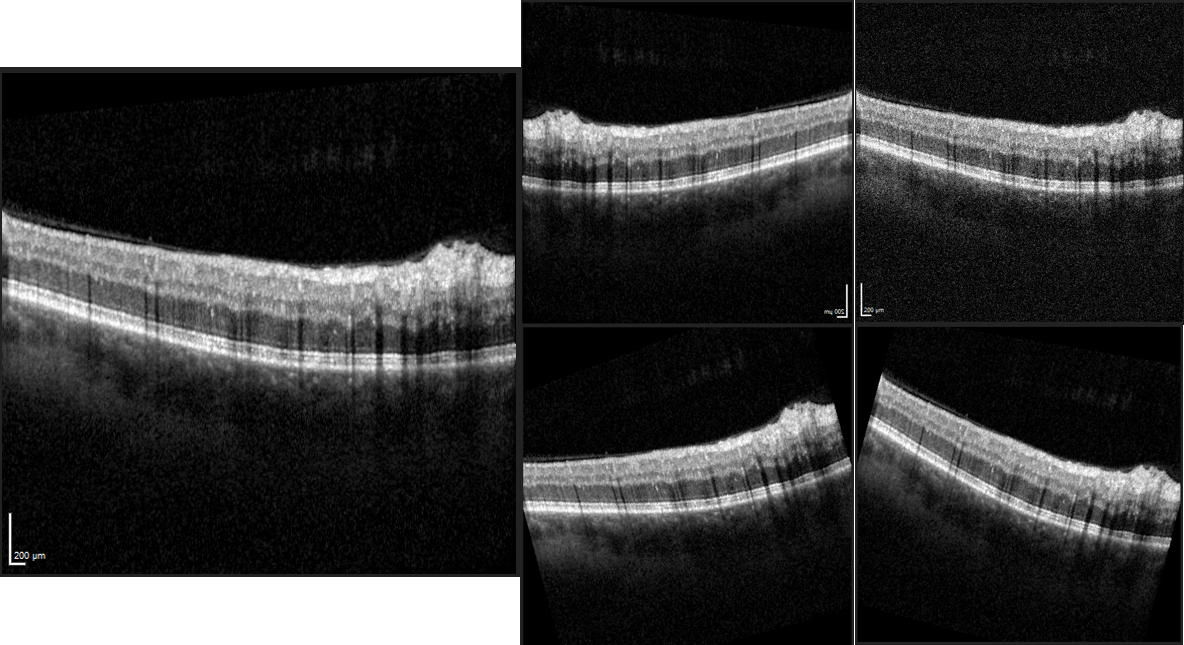
\includegraphics[width=0.5\textwidth]{./pic/Segmentierung/segm_augmentiert.png}
\caption{\label{fig:segm_augmentiert} Bildaugmentierung im Rahmen des Segmentierungstrainings. Links ist das Originalbild zu sehen. Im rechten Viererblock ist links oben die Spiegelung an der Vertikalachse, rechts oben original mit hinzugefügtem Rauschen, links unten Drehung um +15 Grad, rechts unten Drehung um -15 Grad dargestellt.}
\end{figure}


\newpage
\section{Evaluation}
In diesem Kapitel wird das Ergebnis des Segmentierungsmodells anhand der Trainings- und insbesondere Testdaten evaluiert.\newline
Dabei werden sowohl die Kenngrößen bei der Betrachtung des Segmentierungsmodells als binärer Klassifizierer als auch eine feinere Auswertung der Trainings- und Testdaten anhand der Maßzahl IoU vorgestellt.
%%% Strukturnotizen %%%
% IoU
% sensitivity & specificity
% 
\subsection{Segmentierung als binärer Klassifizierer} \label{Segmentierung als binärer Klassifizierer}
%TODO add certainty segmentation
Zu den Ausgabeinformationen der Segmentierung zählen umrandende Boxen ("Bounding Box") sowie Masken gefundener Bereiche. Mithilfe dieser Information kann eine binäre Klassifikation erreicht werden: Wenn mindestens ein Ödem im Bild ermittelt wird und somit mindestens eine Box sicher\footnote{sicher bestimmt gilt ein Ödem, wenn der Parameter \textit{certainty} der zugehörigen Box mindestens 70\% beträgt. Dieser Parameter wurde mithilfe einer Auswertung von Stichproben von uns als passend identifiziert.} bestimmt ist, wird das Bild als "positiv"$\;$klassifiziert. Wenn keine Box sicher ermittelt wurde, wird das Bild als "negativ"$\;$klassifiziert und somit angenommen, dass kein Ödem in dem Bild vorhanden ist.\newline
Insgesamt kann die Evaluation der Klassifizierung auf zwei Ebenen stattfinden: Einerseits auf Bilderebene, bei dem die Klassifikation pro Bild ausgewertet wird. Dabei wird die Auswertung unabhängig von der Zugehörigkeit eines Bildes zum Auge vorgenommen.
Eine weitere Möglichkeit der Evaluation ist die Bewertung auf Augenebene. Dabei wird das Auge eines Patienten, also das Kollektiv aus 25 Bildern, betrachtet. Sobald in mindestens einem Bild der Bilderserie ein Ödem segmentiert wurde, gilt das gesamte Auge als "positiv". \newline
Für diese Evaluation wurden auf Bildebene ausschließlich Testdaten herangezogen, welche nicht im Training gesehen wurden. Somit ergibt sich ein positiver Testdatensatz mit einem Umfang von 50 Bildern, was im Rahmen von Evaluationen eher gering ist. Da dieses Ergebnis somit eine statistische Schätzung mit geringem Stichprobenumfang darstellt, ist dieses Ergebnis in Hinsicht auf die Performanz mit neuen, noch unbekannten Daten im Rahmen des Klinikalltags mit Unsicherheit behaftet.\newline
Wie in Abbildung \ref{fig:barchart_imgeye} erkennbar ist, werden 98\% der Evaluation auf Bildebene korrekt positiv klassifiziert. In absoluten Zahlen wurde somit nur in einem von fünfzig Bildern fälschlicherweise kein Ödem erkannt. \newline
Auf Bilderebene liegt die Falsch-Negativ-Rate bei 9\%, was bei einem Testdatenumfang von 26607 Bildern als aussagekräftig zu bewerten ist.

\begin{figure}[ht!]
\centering
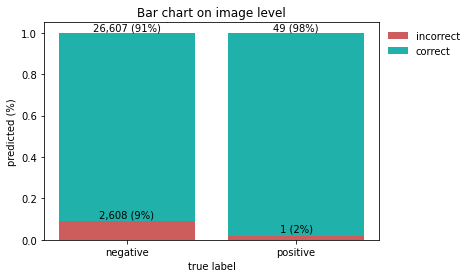
\includegraphics[width=0.49\textwidth]{./pic/Segmentierung/barchart_image.png}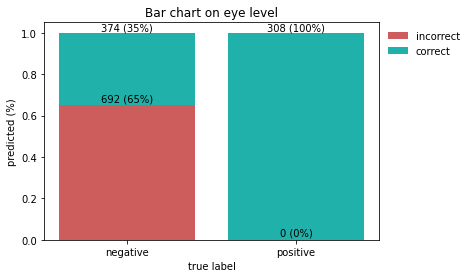
\includegraphics[width=0.49\textwidth]{./pic/Segmentierung/barchart_eye.png}
\caption{\label{fig:barchart_imgeye} Evaluierung der Segmentierung als binärer Klassifizierer auf Bildebene (links) und Augenebene (rechts). Korrekte Klassifikationen sind türkis, inkorrekte rot eingefärbt.}
\end{figure}
Auf Augenebene weichen die Ergebnisse im Vergleich zur Bildebene ab: Alle tatsächlich positiven Augen wurden korrekt als positiv klassifiziert. Dieser Effekt erklärt sich durch die festgelegte Regel, dass bei mindestens einem positiven Bild eines Auges das gesamte Auge als positiv klassifiziert wird, sowie der Tatsache, dass in dieser Evaluation auch Trainingsdaten enthalten sind. 
In dem Szenario der Makulaödemerkennung ist eine Erkennung positiver Fälle wünschenswert: Im Rahmen einer unterstützenden Diagnose ist deutlich schlechter zu bewerten, wenn ein Auge fälschlicherweise als negativ erkannt wird, da somit eine Behandlung des Patienten unter Umständen erst bei einem Folgetermin und somit später als nötig beginnt. Der beste Fall ist es, wenn vorhandene Ödeme stets erkannt werden. Der Anteil von Augen, welcher fälschlicherweise als positiv erkannt wurde, liegt bei etwa 65\%. Eine weitere Untersuchung ergab, dass ein Großteil der falsch positiv klassifizierten Augen aufgrund von zwei oder weniger falsch positiven Bildern fehlklassifiziert wurden.\newline
Diese Ergebnisse führen zu den bereits eingeführten Kennwerten Sensititvität und Spezifität (s. Tab. \ref{tab:sensspec}). Wie auch das Klassifikationsmodell mit Efficient Net wird auch bei der Klassifikation durch das Mask R-CNN eine Sensitivität von 0.98 erreicht. Dabei ist jedoch zu beachten, dass der Wert des Segmentierungsmodells aufgrund des geringen Testdatenumfangs mit Unsicherheit behaftet ist. Darüber hinaus ist die Spezifität des Segmentierungsmodells mit 0.91 sogar besser als jene des Klassifizierers mit 0.82. Aus diesem Grund und aufgrund der Tatsache, dass die Kombination beider Modelle zu tendenziell mehr falsch negativen Fällen führt, wird nur das Segmentierungsmodell in den finalen Prototypen aufgenommen.
\begin{table}[H]
\begin{center}
\begin{tabular}{ l | r | r }
   & Segmentierung Mask R-CNN & Klassifikation Efficient Net \\\hline
 Sensitivität & 0.98 & 0.98 \\  
 Spezifität & 0.91 & 0.82    
\end{tabular}
\caption{\label{tab:sensspec} Sensitivität und Spezifität der Klassifikation auf Bilderebene. Dabei werden die Ergebnisse des Segmentierungsmodells in Funktion eines binären Klassifizierers mit dem Klassifikationsmodell des Efficient Net verglichen.}
\end{center}
\end{table}
% TODO Nachweis
% TODO TO DECIDE schreiben, dass tp eig mist ist?

\subsection{Intersection over Union (IoU)}
Um die Güte eines Segmentierungsresultates zu beschreiben, reichen bisherige Kennzahlen wie Sensitivität und Spezifität nicht aus. Vielmehr muss die Lage und Größe des vom Modell bestimmten Segments mit Lage und Größe des wahren Segments verglichen werden. Eine Kennzahl hierfür ist die Intersection over Union (IoU).
\subsubsection{IoU als Maßzahl}
In diesem Kapitel wird die bereits in Definition \ref{IoU} eingeführte Kenngröße IoU anschaulich gezeigt um die Interpretation der Ergebnisse zu unterstützen.\newline
Im Folgenden wird allgemein von zwei Flächen gesprochen. Auf das Segmentierungsergebnis übertragen repräsentiert eine Fläche die wahre, von Hand segmentierte Fläche und die Andere die Segmentierung des Modells.\newline
Die Intersection over Union wird in Abbildung \ref{fig:iou} visualisiert. Diese setzt den Schnitt beider Flächen, also die gemeinsame Fläche, in das Verhältnis zur Vereinigung. Eine IoU von 1 repräsentiert ein perfektes Ergebnis, bei dem das vom Modell bestimmte Segment exakt dem von Hand markierten Bereich entspricht. Hingegen ist eine IoU von 0 ein Zeichen einer stark fehlerhaften Segmentierung, welche entweder vom Modell an falscher Stelle vorgenommen wurde oder wenn gar kein Segment erkannt worden ist.

\begin{figure}[H]
\centering
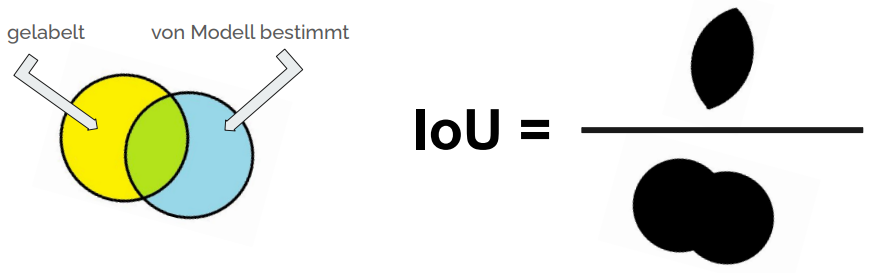
\includegraphics[width=\textwidth]{./pic/Segmentierung/iou.png}
\caption{\label{fig:iou}Zusammensetzung der Kennzahl Intersection over Union (IoU): Dabei wird das Verhältnis von Durchschnitt zu Vereinigung der von Hand segmentierten Fläche und von Modell erkannten Fläche gebildet.}
\end{figure}

Darüber hinaus kann die Aussagekraft der IoU von weiteren Faktoren beeinflusst werden. Eine solcher Einflussfaktor ist die Größe der segmentierten Flächen: Durch das Bilden eines Verhältnisses haben kleine absolute Abweichungen von kleinen Flächen ein höheres Gewicht als bei großen Flächen. Somit ist zu erwarten, dass die IoU bei kleinen Segmenten tendenziell schlechter ausfällt obwohl die subjektive Segmentierungsqualität in etwa gleich wirkt. Somit kann es sinnvoll sein, die Größe bei der Evaluierung der Qualität anhand der IoU zu berücksichtigen. Zudem spielt der Faktor Mensch eine Rolle: Die Segmentierung von Hand wurde von unterschiedlichen Personen durchgeführt. Trotz anfänglicher Absprache kann es auch hier zu unterschiedlichen Arten der händischen Segmentierung kommen. Darüber hinaus wurden die Bilder von Data Science Studierenden und nicht von medizinischem Fachpersonal durchgeführt, weswegen es trotz Hilfestellung von Augenärzten zu Fehlsegmentierungen in den Originalbildern kommen kann.

%TODO remove newpage

\subsubsection{IoU der Trainings- und Testdaten}

Bei einer Auswertung der IoU des Testdatensatzes (Abb. \ref{fig:iou_testonly50}) zeigt sich, dass der Median der IoU bei 0.70 und der Mittelwert bei 0.63 liegt.\newline
Auf einem Testbild wurde kein Segment erkannt, was zu einer IoU von 0 führt.
% TODO mehr ausfuehren
Aufgrund des Umfangs von 50 positiven Testbildern wirkt das Histogramm nicht glatt. Nichtsdestotrotz zeigt sich eine Häufung von Bildern in einem IoU Bereich von 0.4 bis etwa 0.9.

\begin{figure}[H]
\centering
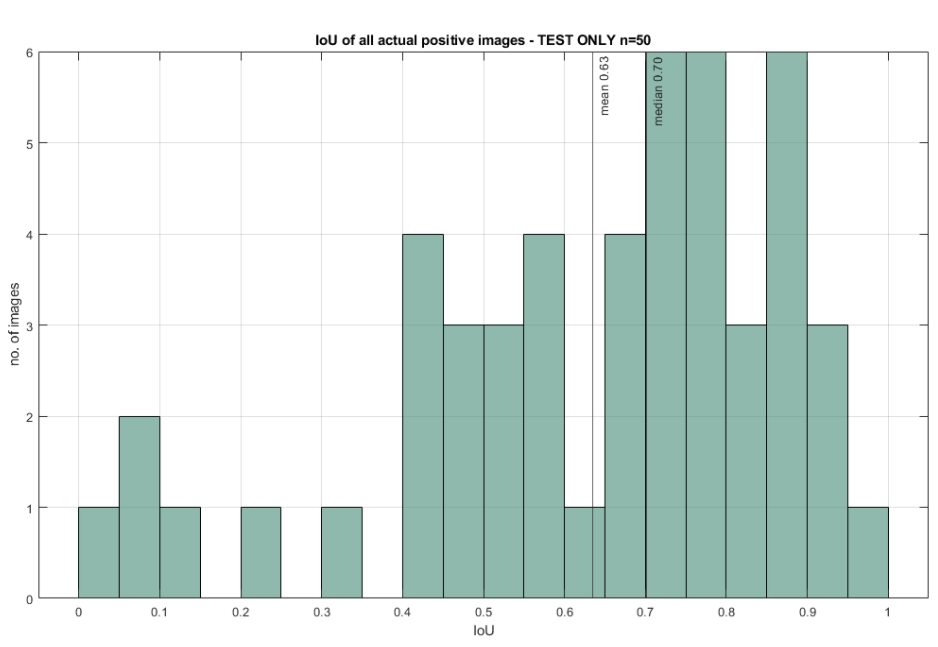
\includegraphics[width=\textwidth]{./pic/Segmentierung/iou_testonly50.png}
\caption{\label{fig:iou_testonly50}Histogramm der Intersection over Union als Ergebnis der Evaluation aller positiven Testdaten. Auf der Abszisse ist die Intersection over Union, auf der Ordinate die Anzahl der Bilder aufgetragen.}
\end{figure}

Im Median liegt bei der Evaluation der positiven Bilder eine IoU von 0.74 vor. Somit wird bei der Hälfte der Ergebnisbilder eine IoU kleiner als 0.74, der anderen Hälfte eine IoU größer als dieser Wert zugeordnet. Wie erwartet, wurde bei keinem Bild eine IoU von 100\% erreicht. \newline

Da der Testdatenumfang mit 50 Bildern gering ist, wurde in einem weiteren Evaluationsschritt neben den Testdaten auch die Trainingsdaten herangezogen. Dabei ist zu beachten, dass diese Ergebnisse eher eine Obergrenze zur Performanz auf neuen, unbekannten Daten darstellen. Das heißt, dass die tatsächliche Performanz des Modelles auf neuen Daten generell schlechter sein wird als die folgenden Bilder zeigen.\newline
Bei der Auswertung von sowohl Trainings- als auch Testdaten (s. Abb. \ref{fig:iou_testonly50})  zeigt sich, dass sowohl Median (0.74) als auch Mittelwert (0.66) etwas höher sind im Vergleich zu der Auswertung der Testdaten. Dieser Effekt ist dadurch erklärbar, dass Trainingsdaten dem Modell bereits bekannt sind und somit tendenziell besser abschneiden. Die Abweichung ist jedoch nicht extrem, was ein Hinweis auf eine gute Performanz des Modells auf unbekannten Daten ist.


\begin{figure}[H]
\centering
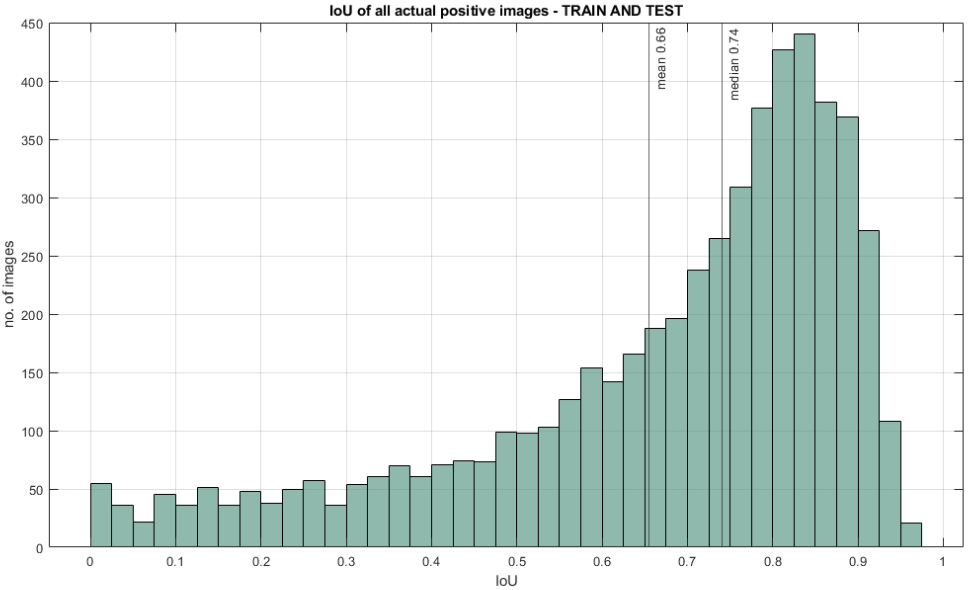
\includegraphics[width=0.8\textwidth]{./pic/Segmentierung/iou_pos_traintest.png}
\caption{\label{fig:iou_pos_traintest}Histogramm der Intersection over Union (IoU) als Ergebnis der Evaluation aller original positiven Bilder. Dabei sind sowohl Trainings- als auch Testbilder berücksichtigt. Auf der Abszisse ist die Intersection over Union, auf der Ordinate die Anzahl der Bilder aufgetragen.}
\end{figure}

Bei einer Betrachtung der Auswertung pro Größenintervall (Abb. \ref{fig:iou_pos_traintest_persize}) werden die zuvor aufgestellten Hypothesen bestätigt: Es zeigt sich, dass die Werte der Lagemaße der IoU bei kleinen Segmenten (weniger und gleich 800 Pixel) geringer sind als bei größeren Ödemen. Darüber hinaus ist die Streuung der im Histogramm dargestellten Verteilungen bei kleinen Segmenten größer als bei mittelgroßen oder großen Segmenten. Das bedeutet nicht zwingend, dass große Ödeme von dem Modell besser segmentiert werden sondern kann auf die Berechnung der IoU zurückgeführt werden.

\begin{figure}[H]
\centering
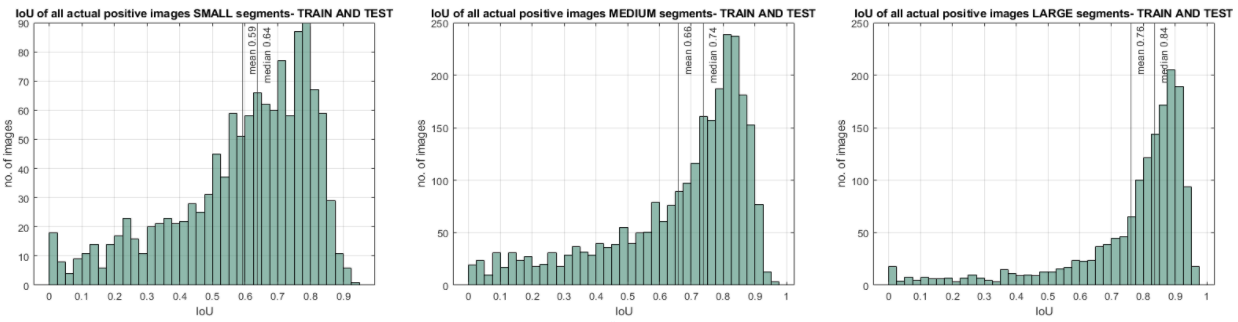
\includegraphics[width=\textwidth]{./pic/Segmentierung/iou_pos_traintest_persize.png}
\caption{\label{fig:iou_pos_traintest_persize}Histogramm der Intersection over Union (IoU) als Ergebnis der Evaluation aller original positiven Bilder. Insgesamt sind drei Histogramme zu sehen, welche sich in der Größe der segmentierten Ödeme unterscheiden. Links ist das Histogramm kleiner Ödeme (kleiner gleich 800 Pixel), in der mittleren Darstellung mittelgroße Ödeme (ab 801 bis 10.000 Pixel), rechts große Ödeme (größer als 10.000 Pixel) dargestellt. Dabei sind sowohl Trainings- als auch Testbilder berücksichtigt. Auf der Abszisse ist die Intersection over Union, auf der Ordinate die Anzahl der Bilder aufgetragen.}
\end{figure}
\newpage
\subsection{Anzahl segmentierter Pixel tatsächlich negativer Bilder}
Da bei tatsächlich negativen Bildern die von Hand segmentierte Fläche nicht vorhanden ist, kann diese Metrik zur feineren Beurteilung der Performance des Modells nicht herangezogen werden. Möglich ist hingegen die Evaluation der Größe fälschlich segmentierter Flächen durch die Anzahl der segmentierten Pixel im Bild.\newline

\begin{figure}[H]
\centering
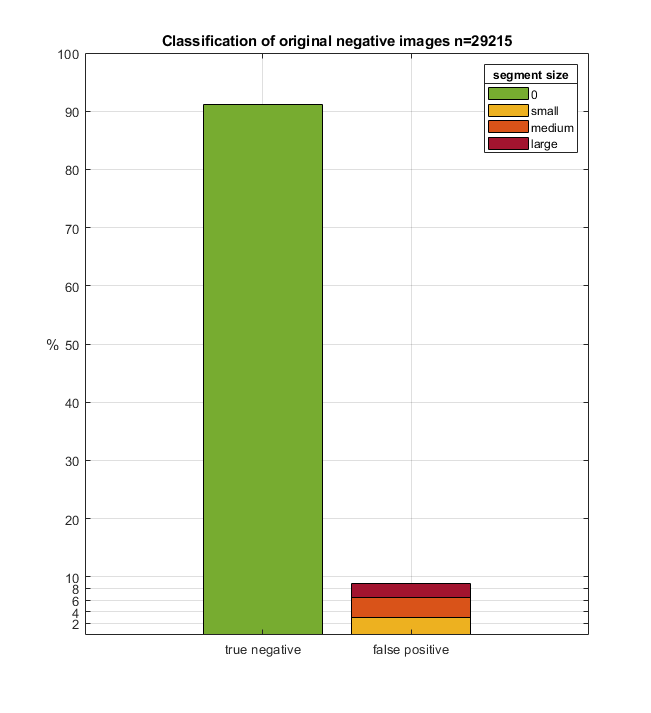
\includegraphics[width=0.7\textwidth]{./pic/Segmentierung/trueNeg_fp_imglevel_n.png}
\caption{\label{fig:trueneg}Darstellung der Anzahl vom Modell segmentierter Pixel tatsächlich negativer Bilder. Links sind die wahren, negativen Bilder dargestellt, rechts alle fälschlich als positiv klassifizierten Bilder. Die Farbcodierung zeigt das Intervall segmentertier Pixel in rot (Größer als 10.000 Pixel), orange (zwischen 800 und 10.000 Pixel) und gelb (weniger als 800 Pixel).}
\end{figure}
In Abb. \ref{fig:trueneg} ist diese Aufteilung visualisiert. Es wird wieder deutlich, dass mit 91\% bei den meisten tatsächlich negativen Bildern vom Modell keine Segmentierung vorgenommen wird. Insgesamt werden in 3\% tatsächlich negativer Bilder kleine Ödeme unter 800 Pixel gefunden, in 4\% der Bilder mittelgroße Ödeme zwischen 800 und 10.000 Pixeln , und in 2\% der Fälle große Ödeme größer als 10.000 Pixel segmentiert.\newline
Diese Information sollte bei der Bewertung der Verlaufskontrolle beachtet werden, da insbesondere große fälschlich erkannte Segmente zu Fehlern in der ermittelten Ödemgröße führen können.


\newpage
\subsection{Auszug von Ergebnisbildern}
Nachdem die Evaluation der Testdaten quantitativ vorgenommen wurde, wird in diesem Kapitel ein Auszug der Testdatenbilder gezeigt. Dabei kann visuell die Größe IoU und die Güte des Segmentierungsergebnisses in Zusammenhang gebracht werden.\newline
Im Folgenden werden die drei Testbilder dargestellt, welche die geringste IoU des Testdatensatzes aufwiesen. In der jeweiligen Teilüberschrift sind die ursprüngliche Bezeichnung des Bildes, die Anzahl vom Modell segmentierter Pixel sowie die berechnete IoU aufgeführt. Rechts wird die Größenklasse angezeigt, in die das vom Modell segmentierte Ödem fällt. Dabei gibt es die Größenklassen 'small', 'medium' und 'large'. Alle drei gezeigten Bilder weisen auf Schwächen des Segmentierungsmodells hin.\newline
In Abb. \ref{fig:ergebnis_notgood1} wurde von dem Modell kein Ödem gefunden. Tatsächlich ist ein Ödem vorhanden. Dieser Fall tritt nur bei einem von den insgesamt 50 Testbildern auf.\newline
\begin{figure}[H]
\centering
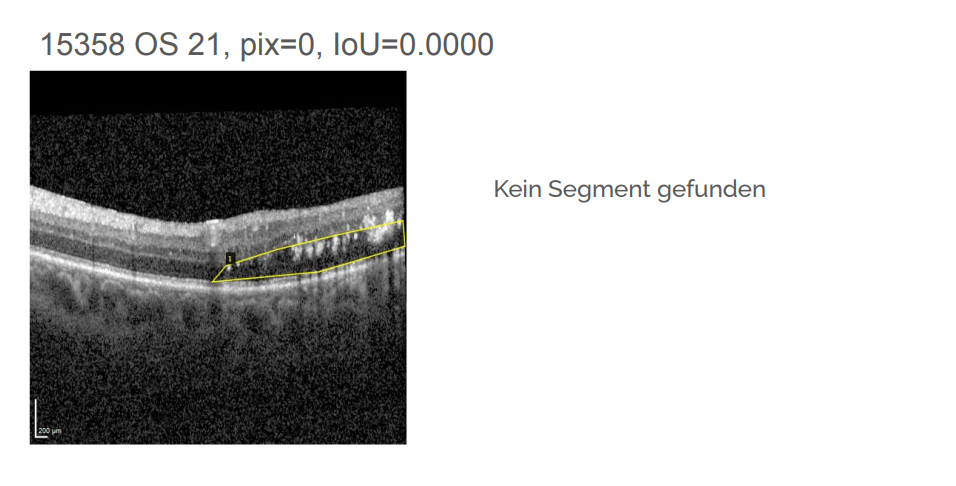
\includegraphics[width=0.75\textwidth]{./pic/Segmentierung/Segmentierungsergebnisse/1.PNG}
\caption{\label{fig:ergebnis_notgood1}Evaluiertes Testbild, bei dem vom Modell Ödem segmentiert wurde. Links von Hand segmentiert, rechts Output des Segmentierungsmodells.}
\end{figure}

Eine weitere Schwäche zeigt sich in Abbildung \ref{fig:ergebnis_notgood2}: Ein kleines Ödem wurde nicht erkannt, dafür aber ein relativ großer Abschnitt einer sichtbaren Hyperreflektivität. Letztere zeichnet sich ähnlich wie ein Ödem durch eine dunklere Abbildung aus, man sieht jedoch, dass die RPE in diesem Bereich ebenfalls dunkler aussieht. Durch gezieltes Training könnte diese Schwäche eliminiert werden. Für die bewertenden Ärzte ist es jedoch von Relevanz zu wissen, dass das Ausmessen solcher Fälle durch das Modell fehlerhaft sein kann.\newline
\begin{figure}[H]
\centering
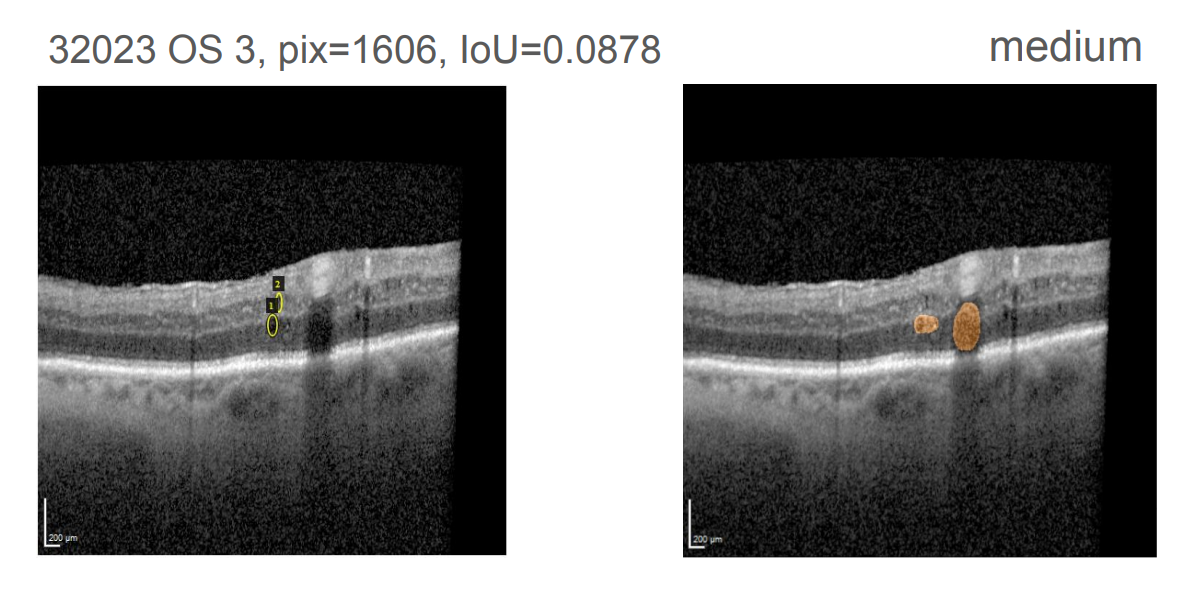
\includegraphics[width=0.75\textwidth]{./pic/Segmentierung/Segmentierungsergebnisse/2.PNG}
\caption{\label{fig:ergebnis_notgood2}Evaluierte Testbild, welches eine geringe IoU und Fehlsegmentierung im Bereich einer Hyperreflektivität aufweist. Links von Hand segmentiert, rechts Output des Segmentierungsmodells.}
\end{figure}

Als dritte Schwäche zeigt sich die fälschliche Markierung eines Ödems unterhalb der RPE, was in Abbildung \ref{fig:ergebnis_notgood3} erkennbar ist. Ein solcher Fehler kann vor Allem in der Ausmessung und somit im Rahmen des Größenverlaufes zu verfälschten Ergebnissen und Missinterpretaitionen führen. Bei weiteren Testbildern mit ähnlicher Abbildung wurden nur Ödeme oberhalb der RPE identifiziert. Dies deutet an, dass der Fehler eher selten vorkommt.\newline
\begin{figure}[H]
\centering
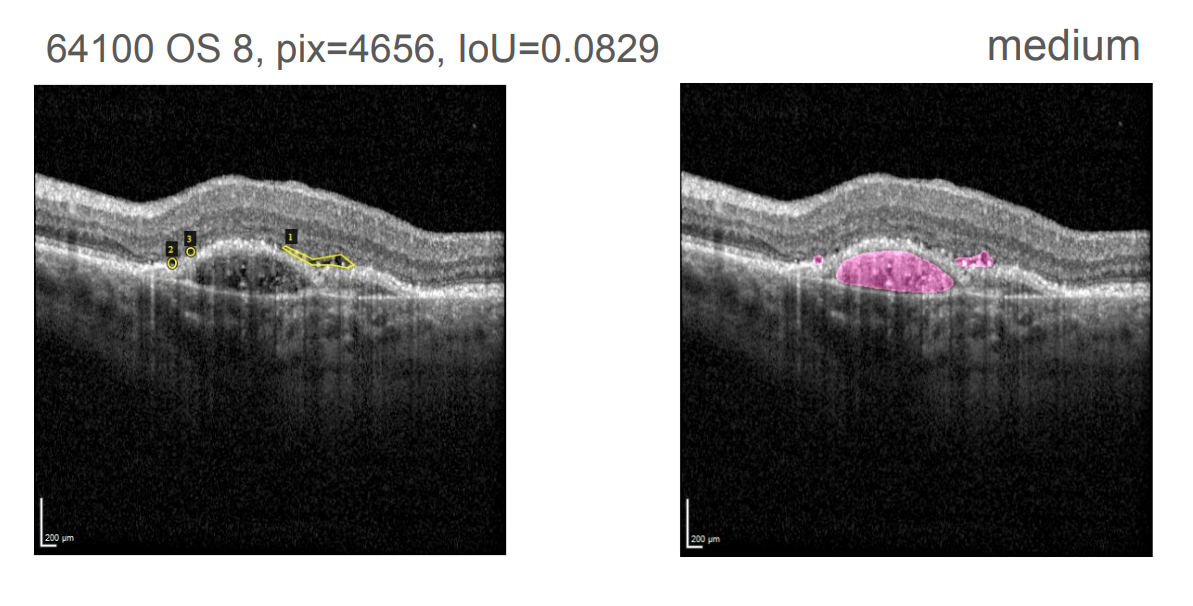
\includegraphics[width=0.75\textwidth]{./pic/Segmentierung/Segmentierungsergebnisse/3.PNG}
\caption{\label{fig:ergebnis_notgood3}Evaluiertes Testbild, welches eine geringe IoU und Fehlsegmentierung aufweist. Links von Hand segmentiert, rechts Output des Segmentierungsmodells.}
\end{figure}

Nachdem eim Auszug der weniger guten Ergebnisse vorgestellt wurde, werden nun Beispiele unterschiedlicher Größen und IoUs gezeigt um einen Eindruck der Resultate der Segmentierung zu gewinnen.\newline
Wieder ist auf der linken Seite jeweils das mithilfe des Image Annotators segmentierte Bild zu sehen, auf der rechten Seite das Ergebnis des Segmentierungsmodells. Dieser Auszug umfasst Bilder mit unterschiedlich großen Segmenten sowie unterschiedlicher IoU.\newline
In Abbildung \ref{fig:ergebnis_good1} ist ein kleines Ödem erkennbar, welches vom Segmentierungsmodell qualitativ gut erkannt wurde. Nichtsdestotrotz ist die IoU mit etwa 0.64 eher im mittleren Bereich einzuordnen. Die geringe IoU kann sowohl aus der geringen Größe resultieren, als auch durch die Verwendung einer Ellipse zur händischen Segmentierung, obwohl das Ödem nicht perfekt elliptisch ist. Fachkräfte stuften dieses Ergebnis im Rahmen der Abschlusspräsentation jedoch als gut ein.
\begin{figure}[h]
\centering
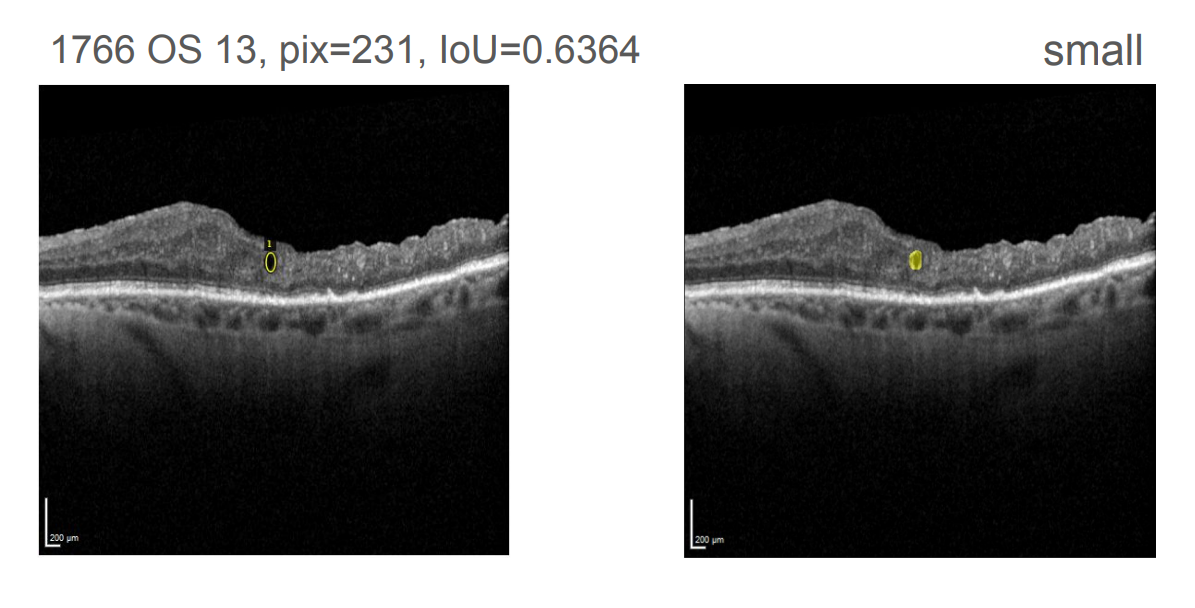
\includegraphics[width=0.75\textwidth]{./pic/Segmentierung/Segmentierungsergebnisse/21.PNG}
\caption{\label{fig:ergebnis_good1}Auszug eines Testbildes, mit einem kleinen Ödem. Links von Hand segmentiert, rechts Output des Segmentierungsmodells}
\end{figure}

In Abbildung \ref{fig:ergebnis_good2} ist ein mittelgroßes Ödem abgebildet, welches sich aus mehreren kleinen Ödemen zusammensetzt. Dies wurde als ein großes Ödem markiert, da die einzeln erkennbaren Flüssigkeitsansammlungen im Gesamtbild auch eine große Flüssigkeitskammer mit kleinen Trennwänden darstellen können. Ähnlich zu der Segmentierung wurde auch die Erkennung und Ausmessung durch das Modell vorgenommen. Bei ähnlichen Bildern zeigt sich, dass in manchen Fällen die schwarzen Flächen einzeln erkannt werden. Diese Unregelmäßigkeit lässt sich wahrscheinlich auf die unterschiedliche Segmentierungsart von Hand zurückführen und muss bei der Bewertung einer Verlaufskontrolle berücksichtigt werden. Da im Rahmen der Verlaufskontrolle stets alle 25 Bilder ins Gewicht fallen und solche Ödeme meist auf mehreren Bildern sichtbar sind, besteht die Möglichkeit, dass dieser Effekt durch die Aufsummierung im Endergebnis abgeschwächt wird.\newline
\begin{figure}[h]
\centering
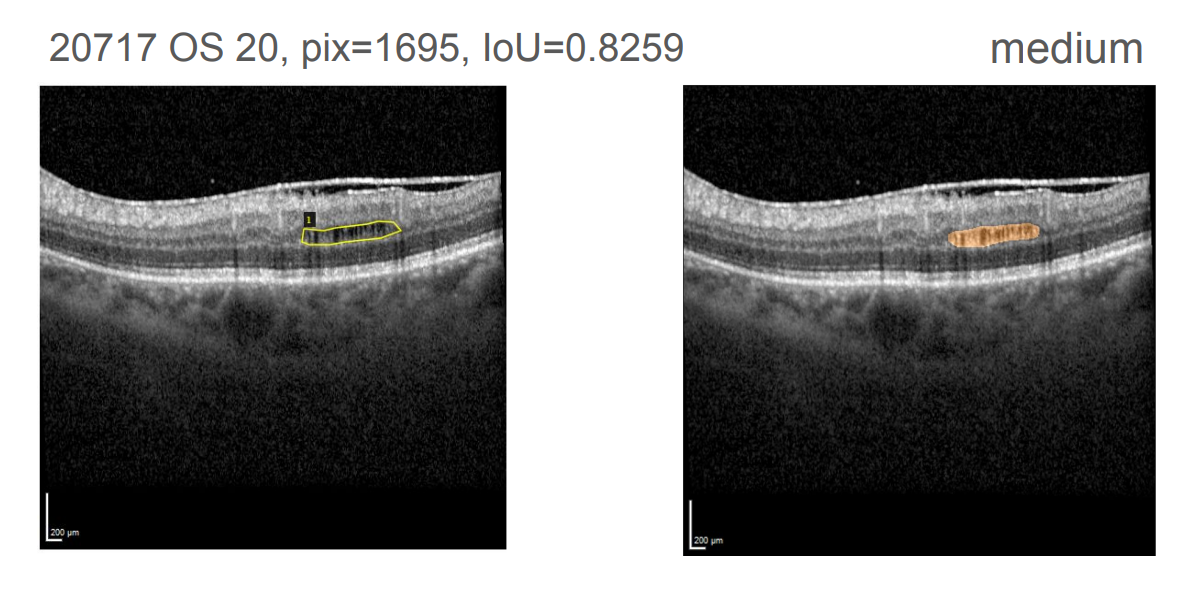
\includegraphics[width=0.75\textwidth]{./pic/Segmentierung/Segmentierungsergebnisse/38.PNG}
\caption{\label{fig:ergebnis_good2}Testbild, welches eine mittlere Größe aufweist. Links von Hand segmentiert, rechts Output des Segmentierungsmodells}
\end{figure}

Ein großes Ödem mit der besten IoU des Testdatensatzes ist in Abbildung \ref{fig:ergebnis_good3} zu sehen. Es zeigt sich eine gute Segmentierung der Fläche durch das Modell, welche so im Rahmen einer Verlaufskontrolle verwendbar wäre. Auch wenn die Ränder nicht immer perfekt getroffen wurden, zeigt sich durch die große absolute Größe des Ödems eine hohe IoU.\newline
\begin{figure}[ht!]
\centering
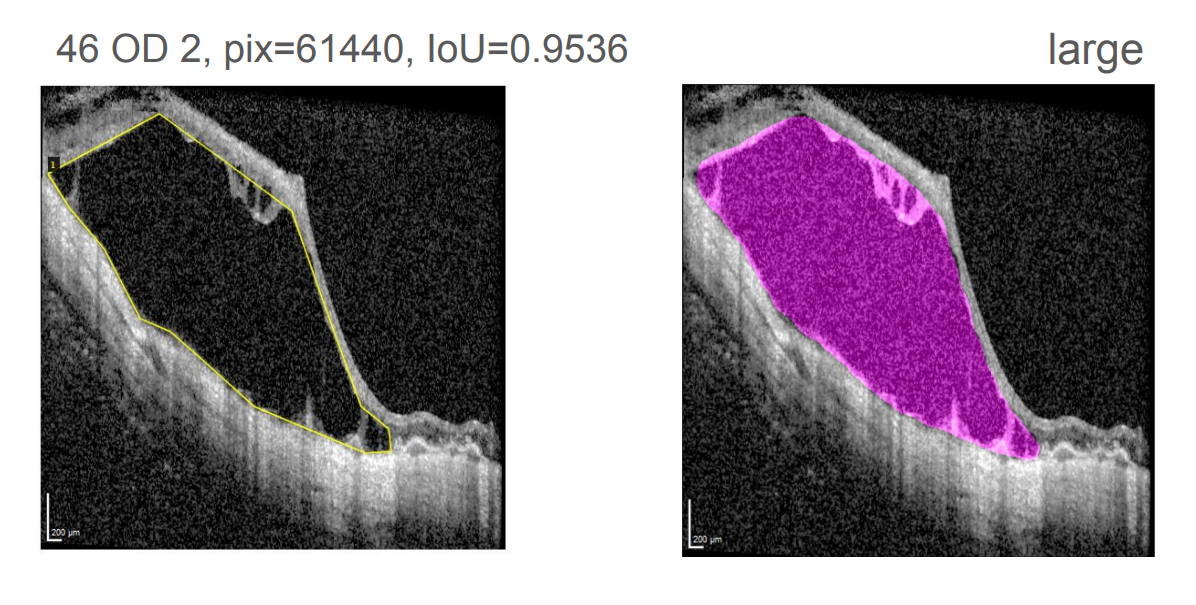
\includegraphics[width=0.75\textwidth]{./pic/Segmentierung/Segmentierungsergebnisse/50.PNG}
\caption{\label{fig:ergebnis_good3}Testbild, auf dem ein großes Segment erkennbar ist. Bei diesem Testbild wurde die höchste IoU erreicht. Links von Hand segmentiert, rechts Output des Segmentierungsmodells}
\end{figure}
Alle Segmentierungsergebnisse der 50 Testbilder befinden sich im Anhang.
%TODO Anhang



\newpage
%TODO remove newpage
\section{Grenzen der Segmentierung und Lösungsvorschläge}

% Häufige Fehler des Modells: ...

% Auf Augenebene hohe Sensitivität, jedoch geringe Spezifität
% Lösung: Einzelne falsch positive Ergebnisse geringer in das Endergebnis einfließen lassen (Spezifitiät verbessern)
Eine Schwäche des Modells ist derzeitig die geringe Spezifität. Wie bereits im Ergebnisteil beschrieben, werden von dem Modell aktuell noch viele der eigentlich negativen Bilder als falsch positive erkannt. 
Um dem entgegen zu wirken, wäre es denkbar einzelne falsch positive Ergebnisse geringer in das Endergebnis einfließen zu lassen. 


% Auswertung der Testdaten ist aufgrund geringer Datenmenge mit Unsicherheit behaftet
% -> Mehr Daten, mehr Training, mehr Test
Bei Deep-Learning-Methoden stellt eine geringe Menge an Testdaten häufig ein Problem dar. 
Da für das Training von dem Gesamtdatensatz nur etwa 5600 Bilder verwendet werden können, wäre es sinnvoll die Menge der Bilder um ein Vielfaches zu erhöhen. Durch das Trainieren des Netzes mit einem umfangreicherem Datensatz, werden robustere Ergebnisse erwartet, die auch die Problematik der geringen Spezifität abfangen sollte. 
Eine weitere Möglichkeit die Menge der Daten zu vervielfältigen ist es die vorhandenen Bilder zu augmentieren. 





\section{Zweites Training des Mask R-CNN}

% Aufgrund der geringen Testmenge: 2. Training mit mehr Testdaten
% 1000 Testbilder
% 4000 Trainingsbilder
% Architektur Modell des MRCNN wurde nich verändert
% -> für repräsentativere Ergebnisse
% leichte Verschlechterung der Ergebnisse
% Training beriets Optimiert -> kein overfitting siehe Grafik. 
% Modell verbessern durch augmentierte Daten

% Da dieses Ergebnis somit eine statistische Schätzung mit geringem Stichprobenumfang darstellt, ist dieses Ergebnis mit Unsicherheit behaftet.
Wie im Unterkapitel \ref{Segmentierung als binärer Klassifizierer} der Evaluierung bereits beschrieben, stellt bei dem trainierten Mask R-CNN Modell derzeit der geringe Stichprobenumfang noch ein Problem bei der Evaluierung dar. Die Ergebnisse sind bei einem zu geringen Testdatensatz noch mit Unsicherheit behaftet. 
Daher wurde das Modell erneut trainiert und dabei nun der Umfang an Testbildern erhöht.
Dabei wurden 1000 OCT-Bilder mit Ödemen dem Trainigsdatensatz entnommen, die später zur Evaluierung genutzt wurden. 
Somit hat sich der Umfang der Daten zum Trainieren des MRCNN-Modells auf 4598 Bilder verringert. Dies führt zwangsläufig zu einer Verschlechterung des Modells. Dafür sind die Ergebnisse dieses Modells aussagekräftiger und robuster. 

Das Vorgehen zum Trainieren des Modells wurde nicht verändert und es wurden die exakt gleichen Parameter verwendet, sodass eine Vergleichbarkeit sichergestellt ist. 
Im folgenden Abschnitt werden die Ergebnisse des zweiten Trainings vorgestellt und zum den Ergebnissen des ersten Modells verglichen. 

In Abbildung \ref{fig:iou_tp_t2} wird die Maßzahl IoU auf den Testdaten gezeigt. 
In dem neu trainierten Modell liegt der Median der IoU bei 0.68 und der Mittelwert bei 0.62.
Zum Vegleich: Im ersten Modell liegt der Median der IoU bei 0.70 und der Mittelwert bei 0.63 (siehe Abbildung \ref{fig:iou_testonly50}).
Somit hat sich das Modell auf Basis der Testdaten nur geringfügig verschlechtert. 




\begin{figure}[H]
\centering
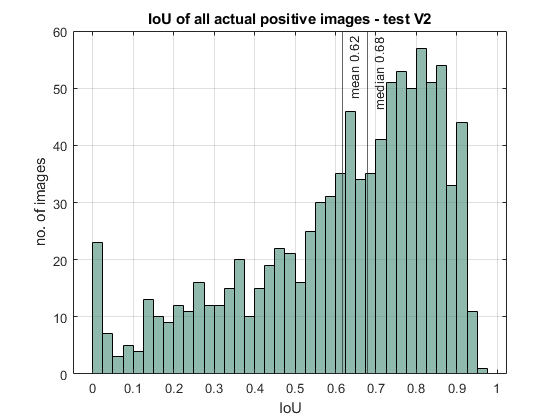
\includegraphics[width=0.7\textwidth]{./pic/Segmentierung/iou_all_tp_train2.png}
\caption{\label{fig:iou_tp_t2}Histogramm der Intersection over Union als Ergebnis der Evaluation aller positiven
Testdaten des zweiten Modells. Auf der Abszisse ist die Intersection over Union, auf der Ordinate die Anzahl der Bilder
aufgetragen. }
\end{figure}


In der nächsten Abbildung wurde wie auch in der Auswertung des ersten Modells die IoU je Ödemgröße ausgewertet. 
Wie auch zuvor schon ist hier zu sehen, dass die Genauigkeit der IoU steigt je größer das zu segmentierte Ödem ist. 
Insgesamt ist aber auch hier wieder eine Verschlechterung um etwa 10\% je Wert zu erkennen. Dabei sinkt die Ungenauigeit mit zunehmender Ödemgröße.



\begin{figure}[H]
\centering
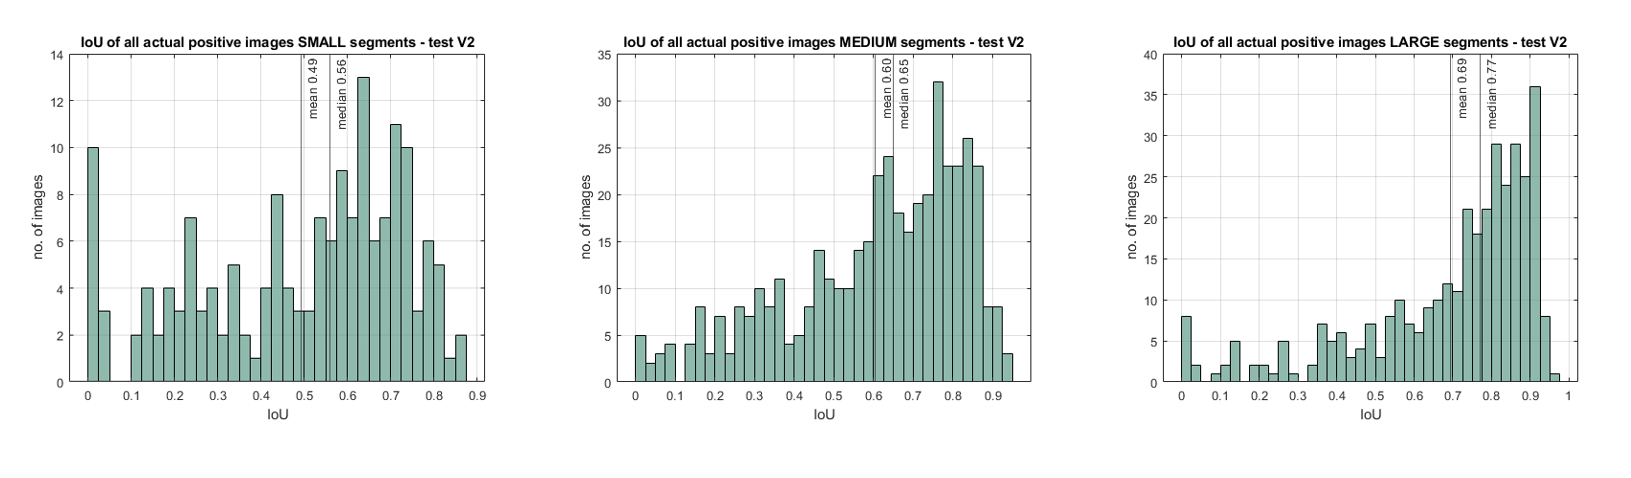
\includegraphics[width=\textwidth]{./pic/Segmentierung/iou_all_sizes_train2.png}
\caption{\label{fig:iou_allsizes_t2}  Histogramm der Intersection over Union (IoU) als Ergebnis der Evaluation aller original positiven Bilder des zweiten Modells. }
\end{figure}


Bei der Auswertung der Performance des neuen Modells auf den negativen Bildern, zeigt sich ein ähnliches Ergebnis. 
Das zweite Modell erreicht eine hohe Spezifität von 90\%. Das ist nur ein Prozentpunkt schlechter als die des ersten Modells. Somit ist die Performance des neu trainierten Modells doch vergleichbar mit dem Vorgängermodell. 
In Abbildung \ref{fig:iou_neg_t2} wird die Rate der richtig und falsch klassifizierten Bildern durch das neue MRCNN-Modell gezeigt. 
Dabei sind die falsch positiven Bilder nach der Größe der gefundenen Ödeme unterteilt. Hierbei ist erneut zu erkennen, dass die Unsicherheit bei kleinen Ödemen größer ist. Kleine (weniger und gleich 800 Pixel) und mittelgroße Ödeme machen einen Anteil von etwa jeweils 4\% unter den falsch positiven aus. Große Ödeme dagegen nur knapp 3\%.




\begin{figure}[H]
\centering
\includegraphics[width=0.6\textwidth]{./pic/Segmentierung/eval_neg_train2.png}
\caption{\label{fig:iou_neg_t2} Balkendiagramm der Anteile richtig und falsch klassifizierter negativen OCT-Bilder des neu trainierten Modells. Links die echt negativ und Rechts die falsch positiv Rate. Die falsch positiv Rate wird unterteilt dargestellt nach Größe der Segmente. }
\end{figure}



Somit hat sich eine Verschlechterung des Modells aufgrund der deutlichen Verkleinerung des Trainingsdatensatzes bestätigt, jedoch fällt diese in einem geringeren Maße aus als erwartet. 
Die mit diesem Modell ermittelten Ergebnisse sind als aussagekräftiger im Vergleich zum ersten Modell zu betrachten. Dennoch beweist die nur geringe Abweichung bereits eine gewisse Robustheit beider Modelle. 



% ---------------------------------------------------------------------------------------------------------
\chapter{Prototyp}
% ----------------------------
In diesem Kapitel wird die Einbettung des erstellten Prototyps zur Erkennung und Ausmessung von Makulaödemen in die Software des Uniklinikums beschrieben.
\section{Architektur}

Die Fidus Software schreibt Ordner mit Patientenbildern auf einen Server.

Das Skript für den Prototypen hat die Aufgabe, zu scannen ob neue Patientenbilder auf dem Server vorhanden sind und wenn ja, diese dem Klassifikationsmodell zu übergeben, deren positiven Output von dem Segmentierungsmodell segmentieren zu lassen um letztlich das Vorhandensein von Ödemen in einem Auge, sowie deren Gesamtgröße, in eine JSON Datei zu schreiben und hinter sich aufzuräumen, indem es die Bilder samt Ordner löscht.

Fidus wiederum verwertet diese JSON Dateien und schreibt die Informationen in die Patientenkartei.

Dieser Workflow ist in Abb. \ref{fig:prototyp} visualisiert. Da wie später in diesem Kapitel beschrieben das Klassifizierungsmodell nicht als Vorfilter verwendet wurde, entfällt der rot dargestellte Teil in der finalen Implementierung.

\begin{figure}[ht!]
\centering
\includegraphics[width=0.75\textwidth]{./pic/Prototyp/flowchart.png} 
\caption{\label{fig:prototyp}Architektur des Skriptes für den Prototypen. - \textit{erstellt mit}: \cite{23}}
\end{figure}

\section{Entscheidung gegen die Klassifikation als Vorfilter}

Die Klassifikation als Vorfilter verbessert in der Theorie die Spezifität, indem sie Möglichkeiten für falsch positive verringert, was in diesem Fall jedoch unerwartet teuer in der Sensitivität schien und weitaus ausführlicher analysiert werden muss, idealerweise mit identischen Trainings- und Testdatensätzen auf beiden Modellen (bei der Segmentierung nur die positiven Bilder dieser Datensätze), um Gewinne in der Spezifität und Verluste in der Sensitivität quantifizieren zu können.

Es fiel auf, dass bei der Evaluation der Klassifikationsmodelle noch mehr Wert auf die Sensitivität gelegt werden sollte, als bereits getan. Das liegt daran, dass selbst wenn beispielsweise zwei Modelle wie in Abbildung \ref{pic:Prefilter_TP} mit einer Sensitivität von 0.9 für sich alleine gestellt recht gut performen, die Kombination dieser wiederum einige echt positive Resultate verliert allein dadurch, dass die 90\% der korrekt positiv klassifizierten des einen Modells nicht zwangsläufig deckungsgleich mit denen des zweiten Modells sind und somit weitere bis zu 10\% Schwund entstehen können. Hierdurch würde man im Gesamtmodell letztlich gerade mal eine Sensitivität zwischen 0.8 und 0.9 erreichen und dementsprechend weniger als nur das Segmentierungsmodell alleine mit seinen 0.9.

\begin{figure}[H]
\centering
\includegraphics[width=0.5\textwidth]{./pic/Prototyp/prefilter.png}
\caption{\label{pic:Prefilter_TP}Der Worst-Case eines Klassifikationsmodells (rot) mit einer Sensitivität von 0.9, eines Segmentierungsmodells (gelb) mit einer Sensitivität von 0.9, sowie die Kombination dieser (blau) mit einer Sensitivität von 0.8, dargestellt als Anteil der echt positiven Bilder (grün). - \textit{erstellt mit}: \cite{23}}
\end{figure}

\section{Umsetzung}

Es gelang eine zufriedenstellende Umsetzung dieser Architektur.

Auf der CPU des Systems der Uniklinik benötigte der Vorgang für 25 Bilder eines Auges in etwa 2 Minuten. Die Ausführung des Skriptes auf dem System der Uniklinik ist in Abbildung \ref{fig:server} zu sehen, die eingebetteten Resultate in die Fidus Software in Abbildung \ref{fig:fidus_beispielpatient}.

\begin{figure}[ht!]
\centering
\includegraphics[width=0.75\textwidth]{./pic/Prototyp/server.png} 
\caption{\label{fig:server}Skript für den Prototypen auf dem Server der Uniklinik}
\end{figure}

\begin{figure}[ht!]
\centering
\includegraphics[width=0.75\textwidth]{./pic/Prototyp/fidus.png} 
\caption{\label{fig:fidus_beispielpatient}Beispielpatient in Fidus}
\end{figure}

\section{Performanceverbesserung des Prototypen}

Mit einer besseren Hardware ließe sich die Dauer der Segmentierung deutlich verkürzen. Mit einer CPU des Typs Intel(R) Core(TM) i5-7500 CPU @ 3.40GHz benötigt man zum Beispiel für 25 Bilder eines Auges etwa 36 Sekunden (Faktor 4) oder mit einer GPU des Typs NVIDIA GeForce GTX 1060 6GB etwa 4 Sekunden (Faktor 34). Insbesondere mit einem Klassifikationsmodell als Vorfilter wäre eine Aufrüstung der Hardware empfehlenswert.






% ---------------------------------------------------------------------------------------------------------
\chapter{Fazit}
% ----------------------------
Die gewählten Modelle und der gewählte Ansatz haben sich als geeignet herausgestellt und die Ergebnisse, die im Rahmen des Projekts erzielt wurden, beweisen bereits eine technische Anwendbarkeit in der Praxis. 
Zudem ist festzustellen, dass alle zu Beginn gesetzten Ziele des Projekts umgesetzt und erreicht wurden.


So erzielt die Klassifikation bereits eine zuverlässige Erkennung von Ödemen auf OCT-Scans mit einer Sensitivität von 0.98 und Spezifität von 0.82.
Darüber hinaus erweist sich auch die Segmentierung als gute Methode zur Erkennung und Ausmessung von Ödemen, was im Rahmen einer Verlaufskontrolle verwendet werden kann. Das Mask R-CNN als binärer Klassifikator weist eine Sensitivität von 0.98 und Spezifität von 0.91 auf. Auf den Testdaten ergab sich eine mediane Intersection over Union von 0.70, wobei der Median bei großen Ödemen höher sowie die Streuung der Verteilung geringer ist. Auch ein weiteres Modell, welches mit mehr Testdaten evaluiert wurde und somit in der Auswertung höhere Aussagekraft hat, zeigt sich ein ähnlicher Median von 0.68.


Insgesamt ist aus technischer Sicht eine gewisse Robustheit der Verfahren und Ergebnisse festzustellen. 
Auch wurde durch den erstellten Prototypen sowohl die technische Machbarkeit sowie Anwendbarkeit in der Praxis demonstriert. Zwar ist im aktuellen Prototypen nur das Segmentierungsmodell enthalten, da ein zweistufiges Verfahren mit separater Klassifikation zu einer geringeren Sensitivität führen würde. Dennoch verspricht eine erfolgreiche Umsetzung mit beiden Methoden in Kombination ein noch besseres Ergebnis. 
Mit der Klassifikation als Vorfilter ist zu erwarten, dass sich die Problematik der hohen Spezifität bei der Segmentierung verbessert.
Daher wäre eine noch genauere vergleichbare Evaluierung und gegebenenfalls Verbesserung des Protoypen mit beiden Verfahren erstrebenswert.  


Eines der Ziele war es eine Verlaufskontrolle zu implementieren, wodurch die Ärzte bei der Diagnostik von Ödemen in Routineuntersuchungen unterstützt werden. Idealerweise würde diese Auswertung den Ärzten später durch ein Programm abgenommen. Der derzeitige Prototyp bietet aktuelle noch keine ausreichende Genauigkeit, als das er die Diagnostik eines Arztes ablösen könnte. Zudem ist neben der Einschätzung des Projektteams auch die Evaluierung der erzielten Ergebnisse durch Mediziner notwendig, um darüber entscheiden zu können, inwiefern sie im medizinischen Kontext bereits anwendbar sind. 

Zudem wurde zum jetzigen Stand eine eher rudimentäre und technische Art der Verlaufskontrolle umgesetzt. Für eine ernsthafte Anwendung in der Praxis, wäre also eine Erweiterung des bisherigen Verfahrens erstrebenswert. Hierfür wäre es von Vorteil einen Ausgabewert gemeinsam mit den Ärzten des Uniklinikums zu entwickeln, der in der Praxis eine verbesserte medizinische Aussagekraft hat. 
Eine erste Idee und mögliche Umsetzung wird im Ausblick erläutert. 









% ---------------------------------------------------------------------------------------------------------
\chapter{Ausblick}
% ----------------------------
In diesem Kapitel wird abschließend ein Ausblick gegeben, wie die umgesetzten Verfahren verbessert oder auch für weitere Projekte erweitert werden könnten. 

Wie im Fazit bereits gesagt, versprechen die Ergebnisse bereits eine Anwendbarkeit in der Praxis. Da sich in diesem Projekt zum ersten Mal mit der Erkennung von Ödemen in Kooperation mit dem Uniklinikum Münster beschäftigt wurde, sind selbstverständlich noch vielerlei Verbesserungen und Erweiterungen denkbar, die im Rahmen dieses Projektes nicht möglich waren. 

Auf einige dieser Aspekte wird im folgenden eingegangen. 

\subsubsection{Datenvorverarbeitung}

Bei weiterer Arbeit an diesem Projekt wäre es für eine Qualitätssteigerung empfehlenswert darauf zu achten, dass mehr Bilder mit Ödemen in den Daten enthalten sind und/oder diese mittels Augmentierungsverfahren dynamisch zu vervielfältigen.

Das Segmentieren der Bilder würde im Idealfall von Experten statt Laien durchgeführt werden, um eine medizinische Korrektheit besser gewährleisten zu können.

Bei mehr als einer segmentierenden Person sollte auch darauf geachtet werden, vorher klare Richtlinien zu formulieren, um die Segmentierung so einheitlich wie möglich zu machen.

Um mit einem Ödem verwechselbare Gegebenheiten wie tote Zellen, Netzhautablösungen oder visuell ähnliche Bereiche unter der RPE besser ausschließen zu können wäre es möglich, diese ebenfalls beim Segmentieren zu markieren und zu lernen, sodass das Netz mehr Informationen mitgeliefert bekommt um diese auseinander zu halten.

\subsubsection{Klassifikation als Vorfilter}

Wie in vorherigen Kapiteln beschrieben versprechen wir uns in der Theorie einen großen Gewinn an Spezifität durch das Klassifikationsmodell als Vorfilter für das Segmentierungsmodell.

Nachdem uns der Effekt des Verlustes an Sensitivität durch Kombination der Modelle bei nicht deckungsgleichen echt positiven Bildern bewusst wurde, sehen wir hier das Gebot einer noch höheren Wertlegung auf die Sensitivität im Klassifikationsmodell, auch auf Kosten der Spezifität dieser, um diesem Effekt entgegen zu wirken und keine kranken Patienten fälschlicherweise als gesund zu deklarieren.

Um den Gewinn an Sensitivität und Verlust an Spezifität genau quantifizieren zu können, sollten Trainings- und Testdatensätze beider Modelle die gleichen sein, wobei die Segmentierung ausschließlich mit den positiven Bildern dieser Datensätze arbeitet.

\subsubsection{Verwendung von augmentierten Daten bei der Segmentierung}
Eine Herausforderung für das Trainings des Mask R-CNN stellte der geringe Datenumfang dar. Methoden zur Augmentierung der Bilder wurden bereits umgesetzt. In Folgeprojekten wäre es daher denkbar, das Problem der geringen Datenmenge durch das Training auf augmentierten Daten zu umgehen.

\subsubsection{Semi-automatisiertes Feedback}

Eine zusätzliche Funktionalität zur Verbesserung der Ergebnisse wäre ein semi-automatisiertes Ärzte Feedback. Hierbei gäben die tatsächlich durchgeführten Behandlungen ein Feedback, welches später mit höherer Gewichtung in ein erneutes Training einfließen könnte, um somit die Genauigkeit kontinuierlich zu verbessern.  

\subsubsection{Erweiterung der Einbindung in Fidus}

Neben der Performanceverbesserung durch Aufrüstung der Hardware stellen wir fest, dass die Ausgabe an Informationen in Fidus momentan mit den Klassen Ödem Ja/Nein und bei Ja, deren Gesamtpixelanzahl sehr beschränkt ist und einer Erweiterung bedarf, um die Ärzte besser bei ihrer Entscheidung zu unterstützen. Einige Beispiele für anzeigbare Informationen:

\begin{itemize}
    \item Die Bilder mit eingezeichneten Segmentierungsflächen
    \item Die Anzahl Bilder auf denen Ödeme gefunden wurden
    \item Wie sicher das Segmentierungsmodell behauptet zu sein
    \item Ein geschätztes Volumen des Ödems anhand Interpolation zwischen den Querschnitten
    \item Eine Einteilung der Ödeme in Größenklassen, welche interpretierbarer als große Pixelanzahlen sein könnten
    \item Eine normierte Gesamtpixelanzahl, um Vergleichbarkeit unabhängig der Anzahl Bilder eines Auges und/oder der Auflösung der Bilder zu schaffen
\end{itemize}

---------------------------
\chapter{Anhang}
% ----------------------------
% TODO include Anhang
\centering
\includegraphics[width=0.9\textwidth]{./pic/Segmentierung/Segmentierungsergebnisse/1.PNG}
\includegraphics[width=0.9\textwidth]{./pic/Segmentierung/Segmentierungsergebnisse/2.PNG}
\includegraphics[width=0.9\textwidth]{./pic/Segmentierung/Segmentierungsergebnisse/3.PNG}
\includegraphics[width=0.9\textwidth]{./pic/Segmentierung/Segmentierungsergebnisse/4.PNG}
\includegraphics[width=0.9\textwidth]{./pic/Segmentierung/Segmentierungsergebnisse/5.PNG}
\includegraphics[width=0.9\textwidth]{./pic/Segmentierung/Segmentierungsergebnisse/6.PNG}
\includegraphics[width=0.9\textwidth]{./pic/Segmentierung/Segmentierungsergebnisse/7.PNG}
\includegraphics[width=0.9\textwidth]{./pic/Segmentierung/Segmentierungsergebnisse/8.PNG}
\includegraphics[width=0.9\textwidth]{./pic/Segmentierung/Segmentierungsergebnisse/9.PNG}
\includegraphics[width=0.9\textwidth]{./pic/Segmentierung/Segmentierungsergebnisse/10.PNG}
\includegraphics[width=0.9\textwidth]{./pic/Segmentierung/Segmentierungsergebnisse/11.PNG}
\includegraphics[width=0.9\textwidth]{./pic/Segmentierung/Segmentierungsergebnisse/12.PNG}
\includegraphics[width=0.9\textwidth]{./pic/Segmentierung/Segmentierungsergebnisse/13.PNG}
\includegraphics[width=0.9\textwidth]{./pic/Segmentierung/Segmentierungsergebnisse/14.PNG}
\includegraphics[width=0.9\textwidth]{./pic/Segmentierung/Segmentierungsergebnisse/15.PNG}
\includegraphics[width=0.9\textwidth]{./pic/Segmentierung/Segmentierungsergebnisse/16.PNG}
\includegraphics[width=0.9\textwidth]{./pic/Segmentierung/Segmentierungsergebnisse/17.PNG}
\includegraphics[width=0.9\textwidth]{./pic/Segmentierung/Segmentierungsergebnisse/18.PNG}
\includegraphics[width=0.9\textwidth]{./pic/Segmentierung/Segmentierungsergebnisse/19.PNG}
\includegraphics[width=0.9\textwidth]{./pic/Segmentierung/Segmentierungsergebnisse/20.PNG}
\includegraphics[width=0.9\textwidth]{./pic/Segmentierung/Segmentierungsergebnisse/21.PNG}
\includegraphics[width=0.9\textwidth]{./pic/Segmentierung/Segmentierungsergebnisse/22.PNG}
\includegraphics[width=0.9\textwidth]{./pic/Segmentierung/Segmentierungsergebnisse/23.PNG}
\includegraphics[width=0.9\textwidth]{./pic/Segmentierung/Segmentierungsergebnisse/24.PNG}
\includegraphics[width=0.9\textwidth]{./pic/Segmentierung/Segmentierungsergebnisse/25.PNG}
\includegraphics[width=0.9\textwidth]{./pic/Segmentierung/Segmentierungsergebnisse/26.PNG}
\includegraphics[width=0.9\textwidth]{./pic/Segmentierung/Segmentierungsergebnisse/27.PNG}
\includegraphics[width=0.9\textwidth]{./pic/Segmentierung/Segmentierungsergebnisse/28.PNG}
\includegraphics[width=0.9\textwidth]{./pic/Segmentierung/Segmentierungsergebnisse/29.PNG}
\includegraphics[width=0.9\textwidth]{./pic/Segmentierung/Segmentierungsergebnisse/30.PNG}
\includegraphics[width=0.9\textwidth]{./pic/Segmentierung/Segmentierungsergebnisse/31.PNG}
\includegraphics[width=0.9\textwidth]{./pic/Segmentierung/Segmentierungsergebnisse/32.PNG}
\includegraphics[width=0.9\textwidth]{./pic/Segmentierung/Segmentierungsergebnisse/33.PNG}
\includegraphics[width=0.9\textwidth]{./pic/Segmentierung/Segmentierungsergebnisse/34.PNG}
\includegraphics[width=0.9\textwidth]{./pic/Segmentierung/Segmentierungsergebnisse/35.PNG}
\includegraphics[width=0.9\textwidth]{./pic/Segmentierung/Segmentierungsergebnisse/36.PNG}
\includegraphics[width=0.9\textwidth]{./pic/Segmentierung/Segmentierungsergebnisse/37.PNG}
\includegraphics[width=0.9\textwidth]{./pic/Segmentierung/Segmentierungsergebnisse/38.PNG}
\includegraphics[width=0.9\textwidth]{./pic/Segmentierung/Segmentierungsergebnisse/39.PNG}
\includegraphics[width=0.9\textwidth]{./pic/Segmentierung/Segmentierungsergebnisse/40.PNG}
\includegraphics[width=0.9\textwidth]{./pic/Segmentierung/Segmentierungsergebnisse/41.PNG}
\includegraphics[width=0.9\textwidth]{./pic/Segmentierung/Segmentierungsergebnisse/42.PNG}
\includegraphics[width=0.9\textwidth]{./pic/Segmentierung/Segmentierungsergebnisse/43.PNG}
\includegraphics[width=0.9\textwidth]{./pic/Segmentierung/Segmentierungsergebnisse/44.PNG}
\includegraphics[width=0.9\textwidth]{./pic/Segmentierung/Segmentierungsergebnisse/45.PNG}
\includegraphics[width=0.9\textwidth]{./pic/Segmentierung/Segmentierungsergebnisse/46.PNG}
\includegraphics[width=0.9\textwidth]{./pic/Segmentierung/Segmentierungsergebnisse/47.PNG}
\includegraphics[width=0.9\textwidth]{./pic/Segmentierung/Segmentierungsergebnisse/48.PNG}
\includegraphics[width=0.9\textwidth]{./pic/Segmentierung/Segmentierungsergebnisse/49.PNG}
\includegraphics[width=0.9\textwidth]{./pic/Segmentierung/Segmentierungsergebnisse/50.PNG}




% ----------------------------
% Bibliography
% ----------------------------

\begin{thebibliography}{}


\bibitem[1]{1} Somit Saha: A Comprehensive Guide to Convolutional Neural Networks - The ELI5 way
 \url{https://towardsdatascience.com/a-comprehensive-guide-to-convolutional-neural-networks-the-eli5-way-3bd2b1164a53} [26.03.2022]

\bibitem[2]{2} ujjwalkarn: An Intuitive Explanation of Convolutional Neural Network
 \url{https://ujjwalkarn.me/2016/08/11/intuitive-explanation-convnets/} [26.03.2022]

\bibitem[3]{3} Rikiya Yamashita et al.: Convolutional neural networks: an overview and application in radiology
 \url{https://insightsimaging.springeropen.com/track/pdf/10.1007/s13244-018-0639-9.pdf} [26.03.2022]

\bibitem[4]{4} Mayank Mishra: Convolutional Neural Networks, Explained 
 \url{https://towardsdatascience.com/convolutional-neural-networks-explained-9cc5188c4939#:~:text=A%20Convolutional%20Neural%20Network%2C%20also,binary%20representation%20of%20visual%20data.} [26.03.2022]

\bibitem[5]{5} Anh H. Reynolds: Convolutional Neural Networks, (CNNs)
 \url{https://anhreynolds.com/blogs/cnn.html} [26.03.2022]
 
\bibitem[6]{6} Daniel Jurafsky, James H. Martin: Chapter 5 Logistische Regression
 \url{https://web.stanford.edu/~jurafsky/slp3/5.pdf#page8} [26.03.2022]


\bibitem[7]{7} Muhammad Tayyab: Mask RCNN \url{https://www.crcv.ucf.edu/wp-content/uploads/2019/03/CAP6412_Spring2018_Mask-RCNN_New.pdf} [26.03.2022]

\bibitem[8]{8} Muhammad Tayyab: Mask RCNN \url{https://www.youtube.com/playlist?list=LL} [26.03.2022]


\bibitem[9]{9} Shaoqing Ren et al.: Faster R-CNN: Towards Real-Time Object Detection with Region Proposal Networks
 \url{https://arxiv.org/pdf/1506.01497.pdf} [26.03.2022]

\bibitem[10]{10} Sambasivarao. K: Region Proposal Network — A detailed view \url{https://towardsdatascience.com/region-proposal-network-a-detailed-view-1305c7875853} [26.03.2022]

\bibitem[11]{11} Tanay Karmakar: Region Proposal Network (RPN)-Backbone of Faster R-CNN \url{https://medium.com/egen/region-proposal-network-rpn-backbone-of-faster-r-cnn-4a744a38d7f9} [26.03.2022]

\bibitem[12]{12} Hyeonwoo Noh et al.: Leaning Deconvolution Network for Semantic Segmentation \url{https://arxiv.org/pdf/1505.04366.pdf} [26.03.2022]

\bibitem[13]{13} Hao Tsui: 2014 Fully Convolutional Network (FCN) Paper summary \url{https://www.youtube.com/watch?v=Ahge3GzQ3Kg&t=887s} [26.03.2022]

\bibitem[14]{14} Connor Shorten: Data Augmentation on Images \url{https://towardsdatascience.com/data-augmentation-and-images-7aca9bd0dbe8} [30.03.2022]

\bibitem[15]{15} AWS: Amazon EC2 P2-Instances \url{https://aws.amazon.com/de/ec2/instance-types/p2/}  [30.03.2022]

\bibitem[16]{16} Tsung-Yi Lin et al.: Microsoft COCO: Common Objects in Context \url{https://arxiv.org/pdf/1405.0312.pdf}  [30.03.2022]


\bibitem[17]{17} nbro: What is a fully convolution network? \url{https://ai.stackexchange.com/questions/21810/what-is-a-fully-convolution-network}  [31.03.2022]

\bibitem[18]{18} Great Learning Team: Fully Convolutional Network (Semantic Segmentation) \url{https://www.mygreatlearning.com/blog/fcn-fully-convolutional-network-semantic-segmentation/}  [31.03.2022]

\bibitem[19]{19} Nicolai Harich: Fully Convolutional Networks for
Semantic Segmentation
from RGB-D images \url{https://hdms.bsz-bw.de/frontdoor/deliver/index/docId/4880/file/master_thesis_fcn_harich.pdf}  [31.03.2022]

\bibitem[20]{20} Nikhil Sardana: Fully Convolutional Networks \url{https://tjmachinelearning.com/lectures/1718/fcn/fcn.pdf}  [31.03.2022]

\bibitem[21]{21} Dive into Deep Learning: 13.10. Transposed Convolution \url{https://d2l.ai/chapter_computer-vision/transposed-conv.html}  [31.03.2022]

\bibitem[22]{22} EffizientNet Pytorch: GitHub \url{https://github.com/lukemelas/EfficientNet-PyTorch} [31.03.2022]

\bibitem[23]{23} draw.io:  Flowchart Maker \& Online Diagram Software \url{https://www.draw.io}

\bibitem[24]{24} VGG Image Annotator \url{https://www.robots.ox.ac.uk/\~vgg/software/via/}

\end{thebibliography}

% ----------------------------
\appendix

% ----------------------------
\end{document}
% ----------------------------
